\documentclass[12pt,a4paper]{report}

% command to compile the file
% xelatex 
% biber 
% xelatex
% choose options for [] as required from the list
% in the Reference Guide, Sect. 2.2
\usepackage{indentfirst}
\usepackage{lipsum}
\usepackage{fancyhdr}
\usepackage{longtable}
\usepackage{makeidx}
\usepackage{hhline}
\usepackage{lastpage}
\usepackage{mathpazo}
\usepackage[svgnames]{xcolor}
\usepackage{pifont}
\usepackage{graphicx}        % standard LaTeX graphics tool
\usepackage{float}  % force the figure at specified location
\usepackage{multirow}
\usepackage{geometry}
\usepackage{diagbox}
\usepackage{rotating}
\usepackage{amsmath}
\usepackage{amssymb}
\usepackage{xeCJK}
\usepackage{longtable}
\usepackage{threeparttable}% tables with footnotes
\usepackage{subfigure}
\usepackage{enumitem}
\usepackage{authoraftertitle}
\usepackage{subfigmat}% matrices of similar subfigures, aka small mulitples
\usepackage{nomencl}
\usepackage{lscape}
\usepackage[hyphens]{url}
\usepackage{caption}

\definecolor{zaffre}{rgb}{0.0, 0.08, 0.66}
\definecolor{azure}{rgb}{0.0, 0.5, 1.0}
	
\usepackage[colorlinks=true, linkcolor=Blue, urlcolor=Maroon, citecolor=Red]{hyperref}
\usepackage[sorting=none,style=numeric,backend=biber]{biblatex}
%\usepackage[ps2pdf, CJKbookmarks=true,bookmarks=true,colorlinks=true,linkcolor=red]{hyperref}

% define a new list with no indent for itemed text
\newlist{dingautolist2}{enumerate}{1}
\setlist[dingautolist2,1]{
  labelindent=\parindent,
  leftmargin=\parindent,
  listparindent=\parindent,
%  labelwidth=2pt,
%  itemsep=2pt,
%  label=(\alph*),
%  label=\protect\circled{\arabic*},
%  label=\protect\textcircled{\small\arabic*},
  label=\protect{\protect\ding{\value*}},
  start=192,
  align=left,
  itemsep=0pt,
  wide=\parindent,
  itemindent=\parindent
%  itemindent=\dimexpr\parindent+\labelwidth+\labelsep\relax
}

%makeindex sample.nlo -s nomencl.ist -o sample.nls
\makeindex

% run gbk2uni *.out file between two runs of latex *.tex

% used for the subject index
% please use the style sprmidx.sty with
% your makeindex program
%%%%%%%%%%%%%%%%%%%%%%%%%%%%%%%%%%%%%%%%%%%%%%%%%%%%%%%%%%%%%%%%%%%\emph{}%%


% Subtract 1 from counters that are used
\renewcommand{\thesection}{\thechapter.\number\numexpr\value{section}\relax}
\renewcommand{\thesubsection}{\thesection.\number\numexpr\value{subsection}\relax}
\renewcommand{\thesubsubsection}{\thesubsection.\number\numexpr\value{subsubsection}\relax}
\setcounter{secnumdepth}{4}


%%%%%%%%%%%%%%%%%%%%%%%%%%%%%%%%%%%%%%%
\graphicspath{{eps/}}
\addbibresource{refs.bib}

\title{飞机全参数化建模方法研究}
\author{宋文滨}
\date{2021年1月20日}

%% the following two lines changes to the Chinese chapter name
\usepackage{titlesec}%chapter1修改为第1章
\titleformat{\chapter}{\raggedright\Huge\bfseries}{第\,\thechapter\,章}{0.5em}{}

% set line spacing
\usepackage[utf8]{inputenc}
\usepackage[english]{babel}
\usepackage{setspace}
\setlength{\parindent}{2em}

\begin{document}
\makeatletter


%\setlength{\parskip}{1em}

%%% set headers 
\pagestyle{fancy}
\lhead{\@title}
\rhead{第\thepage 页/共\pageref{LastPage}页}
\cfoot{上海交通大学}
\renewcommand{\headrulewidth}{0.4pt}
\renewcommand{\footrulewidth}{0.4pt}

%% rename the figure/table to 图/表
\renewcommand{\figurename}{图}
\renewcommand{\tablename}{表}
\renewcommand{\contentsname}{目录}
\renewcommand*\listfigurename{图例}
\renewcommand*\listtablename{表例}
\renewcommand{\bibname}{参考文献}

%%%%%%%title page
\begin{titlepage}
\newcommand{\HRule}{\rule{\linewidth}{0.1mm}} 
\center % Center everything on the page
 
%---------------------------------------------------------------------------------
%     HEADING SECTIONS (Enter the Homework/assignment No., only)
%---------------------------------------------------------------------------------
\textsc{\Large 上海交通大学}\\[0.5cm] % heading course Number
\textsc{\Large 航空航天学院}\\[0.5cm] % heading course name
\textsc{\large \@title}\\[0.5cm] % Minor heading
%---------------------------------------------------------------------------------
%     TITLE SECTION (Replace 'TITLE' with the Homework/assignment Name/title)
%---------------------------------------------------------------------------------
 
\HRule \\[0.4cm]
{ \huge \bfseries \@title}\\[0.1cm] % Title of your Homework/assignment
\HRule \\[1.5cm]
 
%---------------------------------------------------------------------------------
%     AUTHOR SECTION (EDIT THE NAME and T.NO., only)
%---------------------------------------------------------------------------------
 
\begin{minipage}{0.4\textwidth}

\begin{flushleft} \large 
\emph{编写:} 编写\\
\end{flushleft}

\begin{flushleft} \large
\emph{校对:} 校对\\
\end{flushleft}

\begin{flushleft} \large
\emph{审核:} 审核
\end{flushleft} 

\begin{flushleft} \large
\emph{批准:} 批准
\end{flushleft} 

\end{minipage}\\[5cm]

\vspace*{\fill}  % place text at the end of page 
{
\includegraphics[width=0.6\textwidth]{sjtu-logo.eps} \\[1cm]
\large \@date } \\[1cm] % Date, change the \today to a set date if you want to be precise
\vfill % Fill the rest of the page with white-space
\end{titlepage}


\include{GradingRubric}
\tableofcontents          % Required
\listoffigures
\listoftables
\newpage

%%%%%%%%%%%%%%%%
%\begin{CJK*}{UTF8}{gbsn}
%\setcounter{secnumdepth}{3} \setlength{\parindent}{2em}


\date
\maketitle

\newpage
\makenomenclature
%\pdfbookmark[1]{Contents}{table}


\setstretch{1.5}
\setcounter{chapter}{0}
\chapter{绪论}
\section{研究背景}

当前国际地缘政治的快速演变为航空产业全球化的发展战略提出了挑战,产业链分布反映了飞机价值链的现状,不同子系统的技术先进性、成熟度、性能指标、成本和供应链可靠性需要在飞机总体方案的价值函数中加以体现,需要考虑不确定性因素对价值函数的影响对总体方案参数的影响。一方面,飞机各系统的研发中,往往关注其单项技术指标的提升,对飞机总体指标的综合影响需要考虑与其他系统的相互影响。

商用飞机研制是一项系统工程,需要紧密、准确对接市场需求,在技术体系建设,型号飞机的成本控制是一项复杂的工程,要基于全寿命成本的研制成本、单机成本及运营成本进行全面考虑,并在方案设计中对各种因素进行经济性方面的考虑。采用不同指标开展方案优化得到的结果不同。需要更全面分析影响成本的主要因素,需要避免单一指标决策带来的问题,在设计的不同阶段对主要影响参数和因素进行明确,重点突破;结合实际情况制定合理的成本目标。对经济性的认识逐渐得到各级部门和设计人员的重视,现有的方法基本借鉴了西方成熟经济体的估算方法,这些估算方法依托其他制造商的经济性数据,通过拟合方法得到。目前对经济性工作的重视程度不断提高,但仍然缺乏系统的方法和实践,更加缺乏实践积累以及型号验证,所以现有的分析方法难以适用我国的政策、社会经济环境和产业,所以需要探索适合我国商用飞机产业情况,关注模型的发展和数据的积累,将技术发展、型号研制和市场需求通过具有可操作性的分析模型进行关联,以便能够指导工程设计人员和管理决策人员做出最优的决策,能够促进我国民机产业发展的经济性方法和体系。

随着波音公司和巴西航空工业公司创建合资公司,以及空客公司对加拿大庞巴迪公司的并购,商用飞机市场出现前所未有的双寡头垄断格局。波音及空客机型座位数分别覆盖了70-450座和100-550座级的所有机型,在技术、市场和供应链领域对新兴制造商进入市场提出了更大的挑战。中国的商用飞机事业刚刚进入快速发展的初步阶段,建设完整的商用飞机产业的时间其实还很短,我国商用飞机项目的研制仍然缺乏取得市场成功的经验,而成本控制与竞争性分析领域尚缺得到实践检验的方法和体系,客观原因造成不同型号之间的变化较大,经验和数据传递不足,缺少成本经验数据的系统规划和研究,和国外成熟飞机产业相比还有距离。特别是如何在设计参数权衡和优化中如何准确把握飞机的性能指标和经济性指标之间的平衡,尚缺乏可信的工作方法、模型和流程。

飞机系统构成的复杂性和供应链体系的全球性、复杂性导致了在总体方案确定中不仅需要考虑技术因素,还需要考虑经济和商业因素,地缘政治也具有重要的影响作用。飞机制造商,航空公司,MRO,以及金融租赁公司对项目的不同利益追求需要最终反映在客户的需求上,实现产业的高竞争力,构成一个复杂系统的综合决策问题。多层级复杂系统的多目标寻优和决策是系统工程学科研究的重要内容之一,反映在飞机方案设计中,首先需要在飞机总体方案和各子系统层级建立相应的分析模型,实现基于模型的分析、综合和优化。一般而言,各子系统均发展了自身的仿真模型,并用于设计过程中,飞机总体方案也有广泛接受的设计方法,其中的模型大多以经验公式和理论方法为基础,并越来越多的使用高可信度的仿真模型。但是,在飞机总体方案阶段直接使用各子系统的仿真模型既不现实,也不可行,需要结合方案设计需求建立关键子系统价值模型,并与飞机总体方案指标(例如直接使用成本和全寿命周期成本等)进行关联,并将这一方法和总体方案迭代优化相结合。其次,CAE方法在飞机方案设计中的应用不断深入,基于模型的仿真称为系统和部件设计的重要手段,推动了数字样机的发展,这一趋势仍在不断发展,与信息技术和网络技术的进一步融合将实现更加丰富的模型和数据集。但是,在总体方案中采用的模型仍相对简单和宏观,针对传统布局的飞机方案设计在很大程度上仍然依赖几十年来积累得到的经验公式和数据,CAE工具的应用更多体现在设计项目的中后期。

本项研究将现有的总体设计方法与CAD系统实现紧耦合,建立基于CAD的飞机总体方案分析方法,并开展面向飞机总体设计的子系统模型研究,将飞机子系统模型和价值函数相结合,利于实现基于模型的系统工程(Model-Based System Engineering,MBSE)方法与价值驱动设计(Value-Driven Design,VDD)的结合。在飞机项目中贯彻系统工程的理念和实践是改善设计质量和提高设计效率的关键技术之一,如果将系统工程的实践和多学科优化相结合,就形成了价值驱动设计。这一方法和实践与基于模型的系统工程有共同的目标,在具体的技术实施中既有共性,也有差异,基于模型的系统工程方法的侧重点在于强调系统工程的原则与应用,而价值驱动设计更加强调如何确定合理的价值函数,分析影响价值函数变化的因素和参数,以及改善具体的价值指标的途径。

针对飞机典型子系统开展建模和飞机总体方案之间建立定量的参数传递模型,并在主流CAD系统中利用其二次开发能力进行实现,可以在飞机项目早期开展对飞机不同方案的更加准确的评估和权衡分析。价值驱动设计在飞机系统设计、结构设计,部件设计,以及发动机选型中都可以得到应用。例如在总体方案阶段,价值驱动设计有利于更加优化飞机设计方案,明确用户需求在价值函数中的体现,以及如何通过参数分析以及优化实现综合价值的最优化,促进型号、技术和产业的发展。

价值驱动设计将价值函数与基于模型的系统工程方法相结合,而价值函数的定义和选择对方案权衡的结果具有至关重要的影响,价值函数的定义受到市场需求的影响,可以根据不同需求进行差异化的定义,也反映了制造商的发展战略、产品定位等方面的特点,应该既包含常用的DOC等目标函数,也不能仅仅限于现有指标的直接应用,目前文献中提出了一些针对特定应用的价值函数的定义方法,尚缺乏系统的对比分析。这一方法体系不仅仅应该在单一的子系统,部件、结构,分系统,甚至单一的型号项目中进行应用,而应该在整个组织架构和产业链内进行推广。对于方案优化,供应商选择、新技术影响分析,以及产业政策影响分析都具有作用。


\section{相关工作}
基于CAD模型的设计方法随着计算机技术的发展,在飞机设计中得到广泛应用。在CAD模型 中参数化是重要的一环,稳健的参数化有助于提升仿真流程的自动化,降低人为因素的影响,满 足优化设计需求。庞巴迪宇航公司\cite{TARKIAN2008aircraft}开发了基于 CATIA V5的参数化飞机几何建模器,可通过读取设计表的参数重新建模一架飞机。Klimmek等\cite{KLIMMEK2014parametric} 针对全机构型使用参数化建模方法和计算机辅助几何设计开发了结构模型,并分析参数变化对不同目标的影响,实现设计的 快 速 迭 代 。
Hürlimann等\cite{HÜRLIMANN2011mass}扩展了飞机和机翼翼盒几何模型的参数,提供更宽广的设计空间,参数变化可以自动传播至整个模型,有效提升工作效率。余雄庆等\cite{Hujie2012aircraft}根据典型客机机翼的特点,应用CATIA二次开发技术建立参数化的机翼气动外形及结构模型,并用于气动结构多学科优化问题。

在飞机型号发展的过程中,积累了大量的经验和准则。若能重复使用这些设计经验,可以有 效提升飞机的设计能力,基于知识工程的方法便可实现工程经验向规范化设计准则的转化。La Rocca\cite{larocca2011knowledge}在航空领域成功应用基于知识工程的方法,有效支撑了飞机设计及优化。Dorbath等\cite{dorbath2011aknowledge}建 立机翼结构有限元模型生成器,采用了基于知识工程的方法和工程规则,在早期设计阶段便可以 准确分析机翼性能。Tang等\cite{tang2013finite}构建了一种知识驱动的快速有限元建模方法,实现几何模型及有限 元网格的自动划分,有效支撑机翼结构有限元参 数分析和优化设计。


\chapter{价值驱动设计方法}

\section{需求分析}

航空旅行将持续增长,乘客的需求也在变化,除了追求更加安全和经济的指标以外,乘客无论对点到点旅行,WI-FI访问,还是对信息“随时随地”的可获取的个性化需求都对航空公司运输模式产生深远影响,需求的变化需要在飞机方案设计中进行充分考虑。多电技术和PHM技术对飞机方案设计和使用方式也带来了深刻的影响,此项工作将针对需求现状和未来需求的变化,新技术的发展进行分析,并转化为飞机方案的具体设计特征或者设计指标。


\section{飞机全参数化模型}

传统的飞机方案设计一般采用经验公式和理论模型,并在大量历史数据和试验数据的基础上进行,世界主要制造商以及学术机构都发展了不同的方法、工具和系统,也存在一些商用的设计软件。有效使用这些软件和工具设计成功的飞机方案需要丰富的工程经验和对需求的了解。后续机型的发展将越来越依赖CAE模型,在CAE模型基础上开展方案设计的优点包括:1)模型可以更加准确;2)考虑的参数更多;3)对经验公式的依赖降低;4)有利于新构型的设计;但是,也存在一些不利的地方:1)构建模型所需的时间和资源较多;2)缺乏试验数据的验证支撑;3)模型的复杂性提高,灵活性下降;4)涉及的参数较多,相互间大多是非线性关系。本项工作将把飞机方案设计的成熟方法(经过验证的、目前广泛采用的方法)与主流CAD系统相结合,实现包括飞机概念设计模块的全参数定义的飞机CAD模型,可以在CAD系统中完成飞机参数优化和优选。

\subsection{全参数模型的设计方法}

建立的飞机全参数化模型包含机翼、机身、短舱、挂架和起落架模型,如图\ref{fig:ModelOverview}所示。基于自顶向下的建模策略,实现飞机参数向各部件的传递,驱动几何模型的更新。在飞机参数定义中,包括顶层飞机需求的参数定义,并建立输入、输出参数集合。输入参数集中按照专业分为推进、经济性、气动、系统、性能、重量、运营、几何、剩余价值,通过运行VBA程序计算得到输出参数。更新的飞机参数传递至各部件内部,与之关联的几何模型随之更新,从而建立飞机新设计方案的CAD模型,用于开展进一步的分析权衡。

\begin{figure}[hbt!]
\centering
\includegraphics[width=.8\textwidth]{ModelOverview.PNG}
\caption{飞机全参数化模型概览}
\label{fig:ModelOverview}
\end{figure}

\subsection{机翼的参数化定义}

建立的参数化机翼包含巡航构型和起降构型,巡航构型可用于评估流场气动特性,起降构型中包含前缘缝翼、后缘襟翼、扰流板等。首先建立机翼的平面形状,在此基础上建立前缘引导线,通过在展向布置不同的控制剖面翼型,经多截面曲面成形即可得到机翼巡航气动外形,如图\ref{fig:WingAeroShape}所示。控制剖面翼型的参数化定义采用绝对参数和相对参数相结合的方式,有效控制翼型的基本特征。各翼型分属不同的零件,便于后续局部翼型的替换。

\begin{figure}[hbt!]
\centering
\includegraphics[width=.8\textwidth]{WingAeroShape.PNG}
\caption{机翼气动外形}
\label{fig:WingAeroShape}
\end{figure}

起降构型中包含增升装置和扰流板,增升装置分为前缘缝翼、后缘襟翼,二者的具体建模流程与主翼巡航外形类似。通过在机翼的平面形状上确定增升装置的布置,从而限制增升装置的空间位置。由多截面曲面成形增升装置的局部外形,并在主翼上分割出部分曲面,共同组成增升装置的曲面,经封闭曲面得到实体模型。对于扰流板的设计,内翼段布置3块,外翼段布置5块。增升装置和扰流板可绕转轴偏转,实现巡航构型和起降构型的转换,分别如图\ref{fig:WingCruise}和\ref{fig:WingTL}所示。

\begin{figure}[hbt!]
\centering
\includegraphics[width=.8\textwidth]{HiLiftCruise.PNG}
\caption{巡航构型}
\label{fig:WingCruise}
\end{figure}

\begin{figure}[hbt!]
\centering
\includegraphics[width=.8\textwidth]{HiLiftTL.PNG}
\caption{起降构型}
\label{fig:WingTL}
\end{figure}

\subsection{机身的参数化定义}

机身类部件一般为圆筒形,横向截面具有相似的造型规律,因此机身的曲面外形可视为横向截面沿纵向按一定规律拉伸成形。机身参数化方法的总体思路是沿机身纵向布置多个截面,并在机身顶部与底部分别布置纵向引导控制线,通过多截面曲面成形完成机身的参数化建模。核心是各截面和纵向引导线的定义方法采用无量纲和物理参数相结合的综合参数化方法,能够实现对机身外形的准确控制。

\begin{itemize}
    \item[(1)] 机身截面外形定义
\end{itemize}

机身用来装载人员、货物、机载设备等,其横向截面的构型需要全面考虑上述因素。本文整个机身的横向截面共7个,其中等直段的两个截面均为圆形,尾部为一条直线,其它部段截面使用上下两段二次曲线来描述。这里以机身截面编号5的曲线定义为例,如图\ref{fig:FuselageSection}所示,截面分为上下两段二次曲线。每段曲线由两个控制点和两条切线定义,并由一个中间参数进行约束。

\begin{figure}[hbt!]
\centering
\includegraphics[width=.8\textwidth]{FuselageSection.PNG}
\caption{机身截面编号5的曲线定义}
\label{fig:FuselageSection}
\end{figure}

\begin{itemize}
    \item[(2)] 机身纵向引导线定义
\end{itemize}

根据机身的纵向外形轮廓,可将机身部段分为机头段、机头与等直段间的过渡段、等直段、等直段与后体间的过渡段以及后体段。这些部段中除去机头附近曲率变化较大外,其它部段曲线变化较平缓,因此采用二次曲线、样条线和直线段完成纵向引导线的定义。其中机身顶部纵向引导线的机头附近曲线和后体部分采用样条线进行描述,底部纵向引导线的后体部分采用样条线描述,等直段使用直线段描述,其它曲线使用二次曲线进行定义。完成的机身纵向引导控制线如图\ref{fig:FuselageGuideLines}所示。

\begin{figure}[hbt!]
\centering
\includegraphics[width=.8\textwidth]{FuselageGuideLines.PNG}
\caption{机身纵向引导控制线}
\label{fig:FuselageGuideLines}
\end{figure}

\begin{itemize}
    \item[(3)] 翼身整流罩的外形定义
\end{itemize}

翼身整流罩用于连接机身与机翼,可大幅减少机身与机翼连接处的干扰阻力。这里的截面定义使用不过控制点的3D曲线,每条3D曲线需6个控制点。通过多截面曲面成形整流罩的初始外形,然后使用机身曲面切割初始整流罩外形,进而得到最终的整流罩模型,如图\ref{fig:Fairing}所示。建立整流罩的位置与机翼安装位置间的稳健关系,使得整流罩具备针对不同机翼安装位置的自适应能力。

\begin{figure}[hbt!]
\centering
\includegraphics[width=.8\textwidth]{Fairing.PNG}
\caption{翼身整流罩的参数化建模}
\label{fig:Fairing}
\end{figure}

\begin{itemize}
    \item[(4)] 设计结果
\end{itemize}

使用7个参数化的机身截面,2条参数化的纵向引导线,经多截面曲面成形,实现了机身模型的参数化建模,如图\ref{fig:FuselageModel}所示。

\begin{figure}[hbt!]
\centering
\includegraphics[width=.8\textwidth]{FuselageModel.PNG}
\caption{机身的参数化建模}
\label{fig:FuselageModel}
\end{figure}

\subsection{短舱的参数化定义}

发动机短舱曲面外形为旋成体,可在周向布置多个截面,依靠前后缘引导线进行外形控制,通过360°扫掠成形。研究建立了参数化短舱模型,其参数化定义分为两层,一层是框架参数化,用于驱动短舱的整体框架外形;另一层是周向布置的截面参数化。两层参数共同决定短舱的气动外形,实现了短舱模型的参数化。

\begin{itemize}
    \item[(1)] 短舱模型框架的参数化定义
\end{itemize}

首先搭建短舱模型的整体框架,作为后续短舱外形建模的基础,如图\ref{fig:NacelleFramework}所示。基础框架中包含了建模的基准平面、关键定位点的定义等,可驱动短舱模型整体外形的变化。

\begin{figure}[hbt!]
\centering
\includegraphics[width=.8\textwidth]{NacelleFramework.PNG}
\caption{短舱模型基础框架的参数化定义}
\label{fig:NacelleFramework}
\end{figure}

基础框架模型中包含用于短舱扫掠成形的引导线定义,引导线可分为前缘引导线和后缘引导线,如图\ref{fig:NacelleGuideLines}所示。因短舱后缘具有厚度,因此分为短舱外表面后缘引导线和内表面后缘引导线。在图\ref{fig:NacelleGuideLines}中后缘引导线有两条,后缘厚度较小,使得不易辨别。引导线的定义使用样条线,前缘引导线和后缘内外表面的引导线均使用8个点进行定义,建立样条线。

\begin{figure}[hbt!]
\centering
\includegraphics[width=.8\textwidth]{NacelleGuideLines.PNG}
\caption{短舱的前缘和后缘引导线}
\label{fig:NacelleGuideLines}
\end{figure}

\begin{itemize}
    \item[(2)] 短舱截面外形定义
\end{itemize}

短舱在周向共布置8个截面,如图\ref{fig:NacelleSections}所示,其中独立截面共5个,截面6、7、8分别是截面4、3、2关于中心平面的对称结果。短舱截面与翼型类似,其参数化定义使用不过控制点的3D曲线。

\begin{figure}[hbt!]
\centering
\includegraphics[width=.8\textwidth]{NacelleSections.PNG}
\caption{短舱周向布置的8个截面}
\label{fig:NacelleSections}
\end{figure}

\begin{itemize}
    \item[(3)] 设计结果
\end{itemize}

将8个短舱截面的上、下翼型作为剖面,前缘引导线和后缘引导线作为扫掠引导线,经扫掠成形得到短舱的外表面和内表面,如图\ref{fig:NacelleModel}所示。模型中的框架外形和纵向截面包含稳健的参数定义,实现了短舱模型的参数化建模。

\begin{figure}[hbt!]
\centering
\includegraphics[width=.8\textwidth]{NacelleModel.PNG}
\caption{短舱的气动外形模型}
\label{fig:NacelleModel}
\end{figure}

\subsection{挂架的参数化定义}

\begin{itemize}
    \item[(1)] 挂架截面外形定义
\end{itemize}

挂架用于连接发动机短舱与机翼下表面,其位置应该随发动机安装位置变化而具备相应的自适应能力。这里采用定义4个截面,通过多截面曲面成形完成挂架的初步建模,如图\ref{fig:Pylon1}所示。每个截面使用多个控制点生成3D曲线,其中截面1和截面4需要7个控制点,截面2和截面3需要17个点。因为挂架外形具有对称性,实际控制参数可以减半,只需建立单侧控制点,然后使用对称命令建立另一侧的控制点。控制点的坐标参数与短舱及机翼的参数相关联,从而使挂架模型具备较强的鲁棒性。

\begin{figure}[hbt!]
\centering
\includegraphics[width=.8\textwidth]{Pylon1.PNG}
\caption{挂架气动外形的初步建模}
\label{fig:Pylon1}
\end{figure}

\begin{itemize}
    \item[(2)] 设计结果
\end{itemize}

完成挂架气动外形的初步建模后,分别使用机翼及短舱的曲面外形分割挂架原始外形,从而得到最终的挂架参数化模型,如图\ref{fig:Pylon2}所示。

\begin{figure}[hbt!]
\centering
\includegraphics[width=.8\textwidth]{Pylon2.PNG}
\caption{挂架的参数化模型}
\label{fig:Pylon2}
\end{figure}

\subsection{基于CAD参数化模型的飞机总体方案分析模块}
CAD工具通常用于从初步设计到后续的设计过程中,由于在快速定参的过程中管理构建和模型更改的复杂性方面存在挑战,因此在概念设计阶段通常不会使用CAD工具,这解释了在飞机参数研究中缺少使用CAD的原因。这项工作采用了相反的方法来将飞机的参数调整功能利用CAD系统中的知识工程功能引入CAD系统。知识工程是人工智能在知识信息处理方面的发展,它主要研究如何由计算机表示知识,进行问题的智能求解。在参数化设计中引入知识工程使得产品的参数值及参数之间的关系可以随一定条件做适当变化,可以将设计中的所有信息集合起来,形成一套详细且灵活的设计方法。

将飞机/发动机概念设计涉及到的所有几何外形参数、气动参数、重量参数、经济性参数、性能参数、运营参数、和发动机的参数,按照飞机的分系统进行分级,通过CAD软件中的知识工程建模(Knowledge advisor)工具,建立参数树,将定义一架飞机的所有参数集成到CAD系统中,并将飞机参数确定程序中使用的几何参数与飞机的3D模型的外形参数直接关联。同时允许通过电子表格直接进行参数化模型的调整。实现这种无缝集成的优点是可以轻松提供详细的几何图形,以便使用更高保真度的工具进行后续分析。

采用基于CATIA的建模方法的框架如图\ref{fig-catiaintegration}所示,该图给出了建模方法的三个主要组成部分,其一是飞机/发动机的几何模型定义;其二为定义飞机和发动机方案的参数集,参数集按照输入和输出两类参数进行组织,在输入和输出参数集中,又分别按照飞机方案设计中的专业模块对参数进行了分组;第三个部分是飞机总体方案设计方法的VBA程序实现,这些方法同样按照不同专业进行分组,形成了模块化的设计工具。模型的三个部分是相互关联的,输入参数定义了飞机的方案,输出参数中给出了飞机设计各个模块的计算结果。

毫无疑问,飞机外形建模在飞机研制过程的不同阶段对外形的细节要求不同,涉及到的参数类型和数目随着设计进展不断增多,在概念方案设计阶段使用的参数数目相对较少,但对飞机方案的总体指标影响深远,将飞机方案设计方法,也就是基于半经验的方法与较为详细的几何定义结合起来,有助于实现快速的方案迭代和尽可能详细的几何信息组合起来,飞机方案的快速迭代的结果可以反映在飞机外形的更新上,
\begin{figure}[htp]
    \centering
   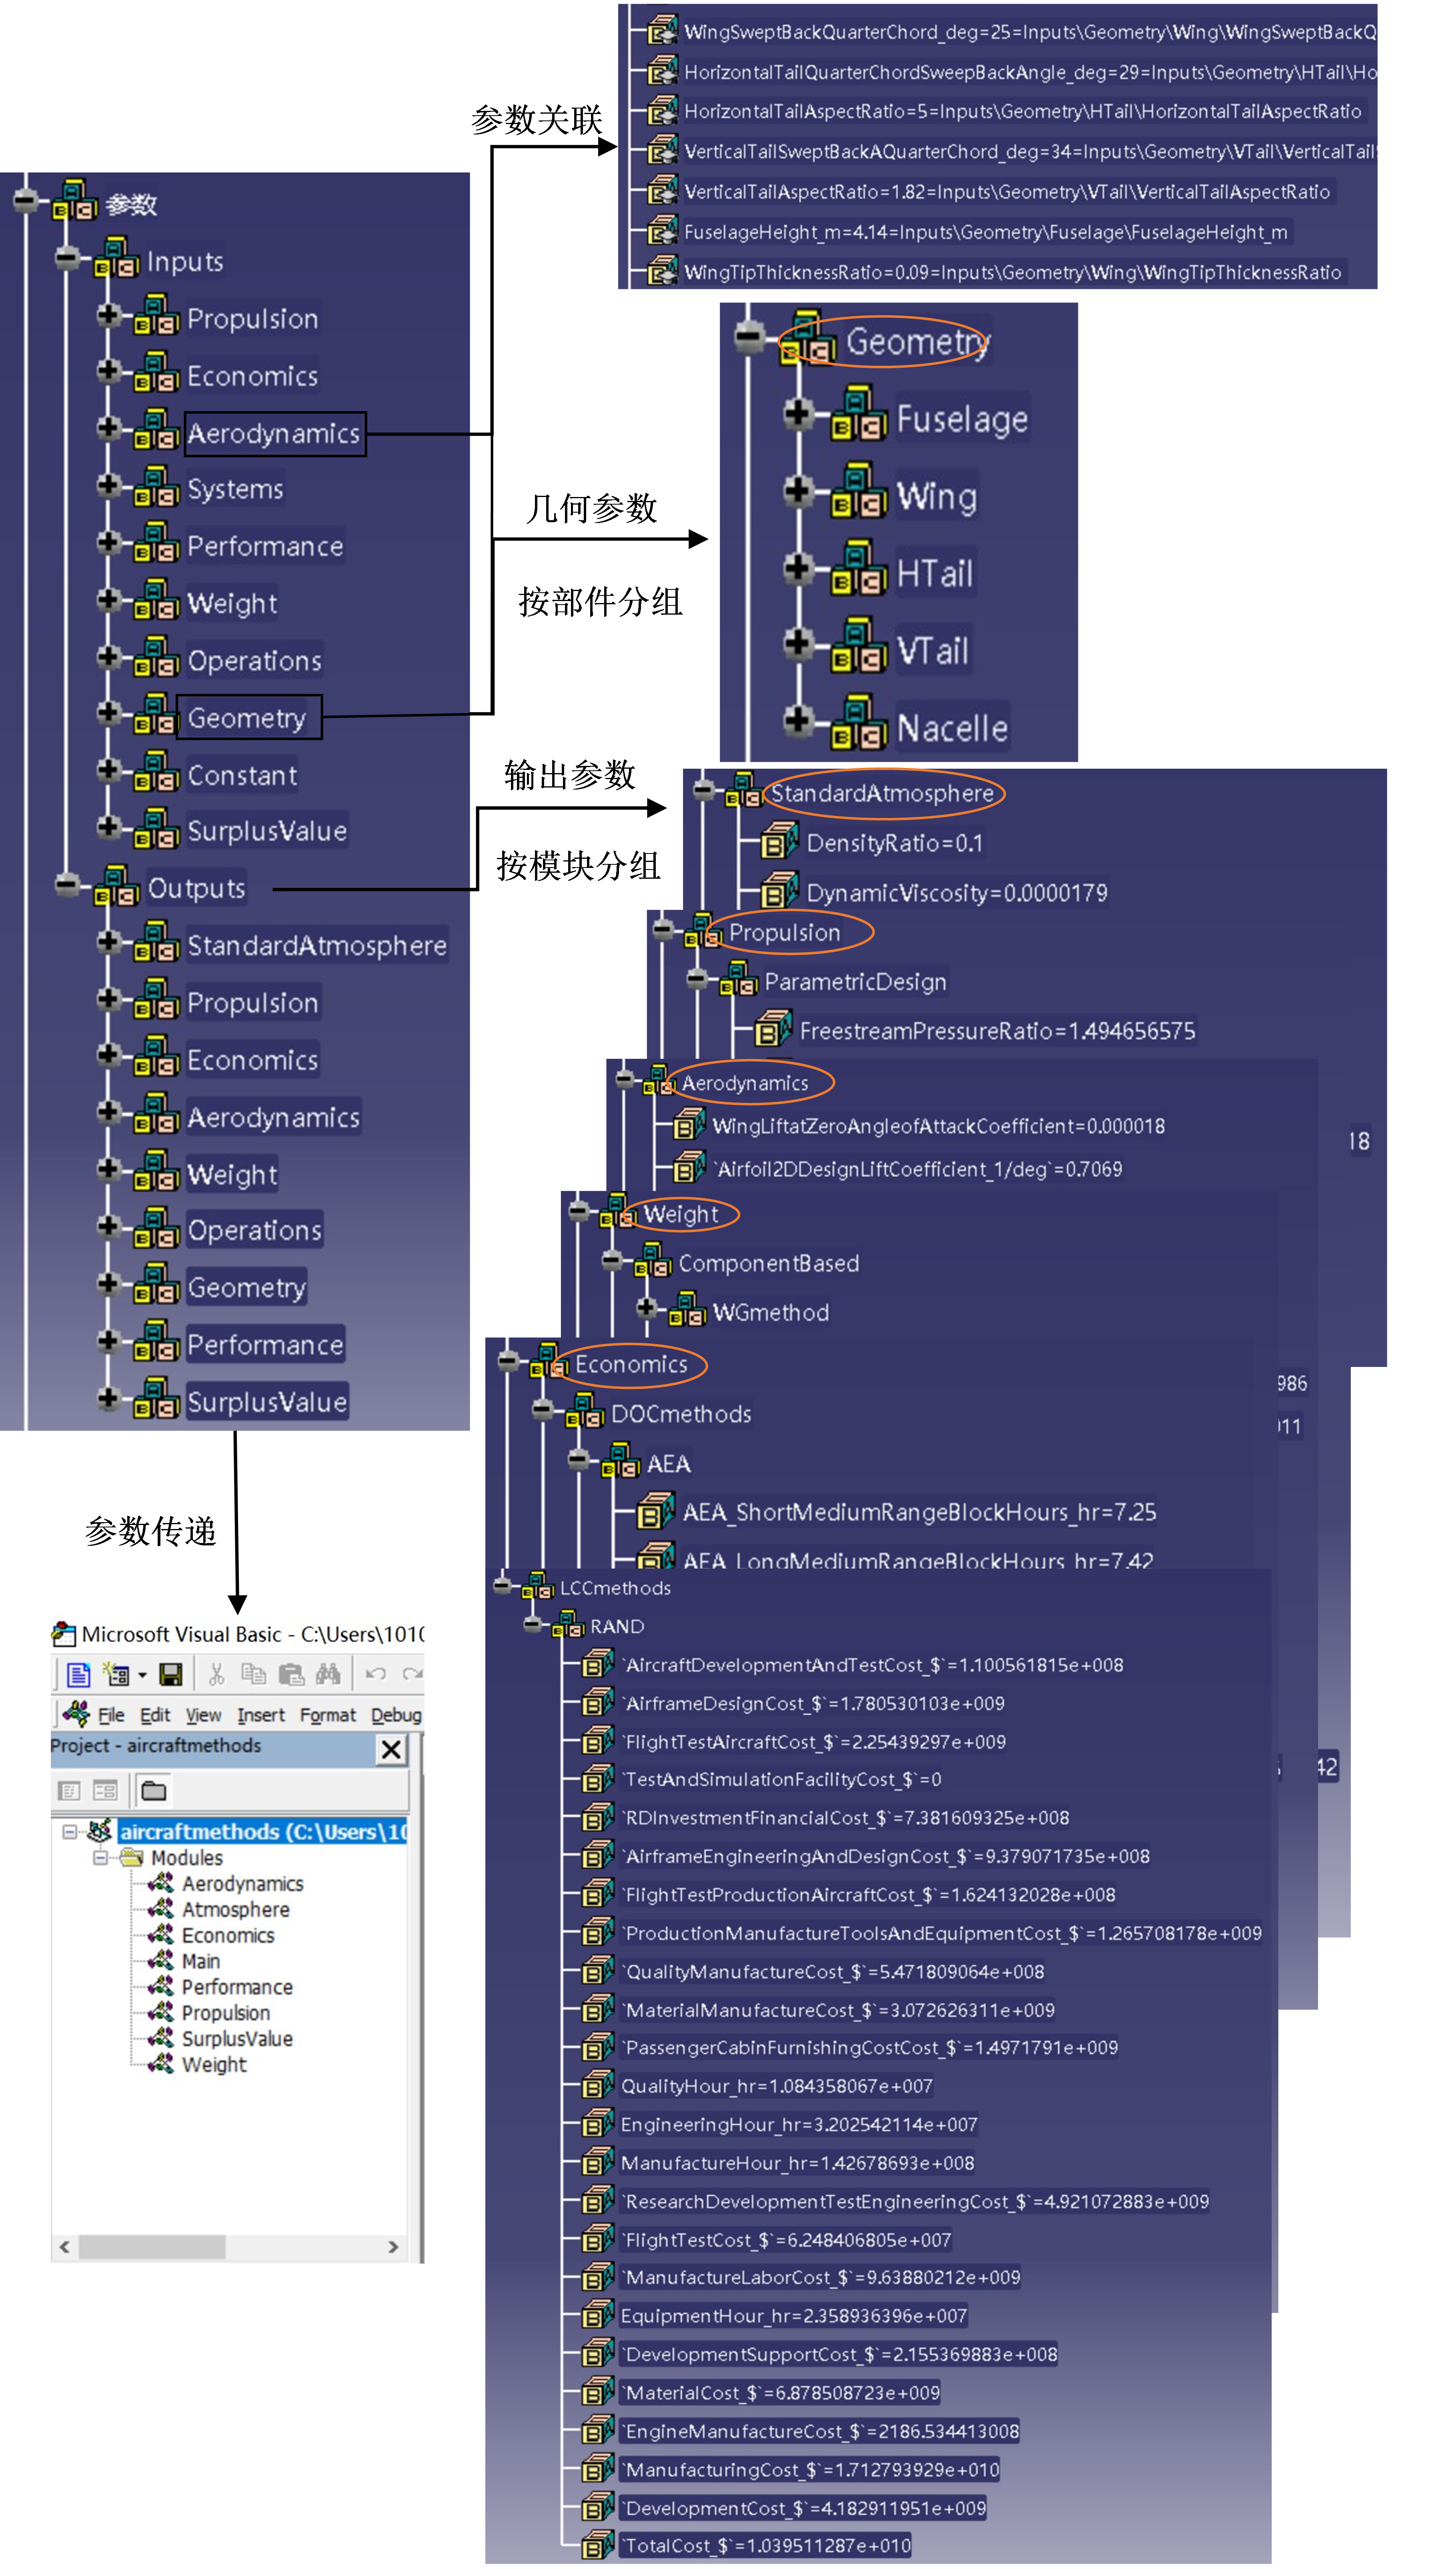
\includegraphics[width=.8\textwidth,height=20cm]{eps/CatiaWorkflow.png}
    \caption{基于CATIA的飞机/发动机一体化建模框架}
    \label{fig-catiaintegration}
\end{figure}

下面将按照不同的分组将定义飞机和发动机的所有参数,按照不同模块分别给出。
\begin{itemize}
    \item[(1)] 发动机模块
\end{itemize}

\begin{center}
\begin{longtable}{|p{5.8cm}|p{3.9cm}|p{1.9cm}|p{1.4cm}|}
\caption{发动机模块的输入参数列表}
\label{tab:engineinput} \\ \hline \hline
\multicolumn{1}{|l|}{参数名称} & \multicolumn{1}{l|}{参数说明} & \multicolumn{1}{l|}{数值}  & \multicolumn{1}{l|}{单位} \\ \hline 
\endfirsthead

\multicolumn{4}{c}%
{{\tablename\ \thetable{} -- 续前页}} \\ \hline \hline
\multicolumn{1}{|l|}{参数名称} & \multicolumn{1}{l|}{参数说明} & \multicolumn{1}{l|}{数值}  & \multicolumn{1}{l|}{单位} \\ \hline 
\endhead
\hline \multicolumn{4}{r}{{下页续}}\\
\endfoot
\hline 
\endlastfoot
MachNumber	&飞行马赫数	&0.78 &-\\\hline
GeometryAltitude	&飞行高度&	10068&m \\\hline
SpecificHeatRatio1	&	燃烧室上游比热容比&	1.4&- \\\hline
SpecificHeatRatio2	&燃烧室下游比热容比&	1.33&-\\\hline
SpecificHeatatConstantPressure1	&燃烧室上游恒压比热容&1.004 & kJ/(kg·K)\\\hline
SpecificHeatatConstantPressure2&燃烧室下游恒压比热容&1.2351&kJ/(kg·K)\\\hline
NewtonConstant	&牛顿常数&	1&(kg·m)/(N·s2)\\\hline
FanPressureRatio	&风扇压比&	1.55&-\\\hline
BurnerExitTotalTemperature	&燃烧室出口总温	&1560&K\\\hline
CompressorPressureRatio	&压缩机压比&15&-\\\hline
DiffuserPressureRatio	&扩散器压比&	0.99&-\\\hline
BurnerPressureRatio	&燃烧室压比	&0.95& -\\\hline
NozzleCorePressureRatio	&	内涵喷管压比&	0.99&-\\\hline
NozzleFanPressureRatio	&	外涵喷管压比&	0.98&-\\\hline
CompressorPolytropicEfficiency	&压缩机多变效率	&0.9&-\\\hline
FanPolytropicEfficiency	&风扇多变效率&	0.89&-\\\hline
TurbinePolytropicEfficiency	&	涡轮多变效率&	0.9&-\\\hline
BurnerEfficiency	&燃烧室效率&	0.99&-\\\hline
BPR	&	涵道比	&5.7&-\\\hline
FuelHeatingValue&	燃料低热值&	42800&	kJ/kg\\\hline
MechanicalEfficiency&	机械效率&	0.99&-\\\hline
PressureRatio9	&环境压力/内涵喷管压力&	1&-\\\hline
PressureRatio19	&	环境压力/外涵喷管压力&	1&-\\\hline
\hline
\end{longtable}
\end{center}

% \begin{table}[ht]\centering
% \caption{发动机模块的输出参数列表}
% \label{tab:engineoutput}
% \begin{tabular}{|p{5.3cm}|p{3.9cm}|p{1.4cm}|p{2.4cm}|}
% \hline \hline
% 参数名称&参数说明&数值&单位\\\hline

\begin{center}
\begin{longtable}{|p{5.8cm}|p{3.9cm}|p{1.9cm}|p{1.4cm}|}
\caption{发动机模块的输出参数列表}{Output parameters of engine module}
\label{tab:engineoutput} \\ \hline \hline
\multicolumn{1}{|l|}{参数名称} & \multicolumn{1}{l|}{参数说明} & \multicolumn{1}{l|}{数值}  & \multicolumn{1}{l|}{单位} \\ \hline 
\endfirsthead

\multicolumn{4}{c}%
{{\tablename\ \thetable{} -- 续前页}} \\ \hline \hline
\multicolumn{1}{|l|}{参数名称} & \multicolumn{1}{l|}{参数说明} & \multicolumn{1}{l|}{数值}  & \multicolumn{1}{l|}{单位} \\ \hline 
\endhead
\hline \multicolumn{4}{r}{{下页续}}\\
\endfoot
\hline 
\endlastfoot
GasConstant1&燃烧室上游气体常数&0.2871& kJ/(kg·K)\\\hline
GasConstant2&燃烧室下游气体常数&0.3065&kJ/(kg·K)\\\hline
SpeedofSound&声速&294.97& m/s\\\hline
AmbientTemperature&大气温度& 288.15&K\\\hline
FlightSpeed & 飞行速度 & 235.98 &m/s\\\hline
FreestreamPressureRatio & 自由流压比 & 1 &-\\\hline
AmbientPressure &环境压力 & 22632&Pa\\\hline
BurnerEnthalpyRatio&燃烧室焓比& 6.651&-\\\hline
FreestreamEnthalpyRatio& 自由流焓比&1 &-\\\hline
FanTemperatureRatio&风扇温比&1.1857 &-\\\hline
FanNozzlePressureRatio& 外涵喷管压比& 2.2601&-\\\hline
MachNumber19&外涵马赫数&1.1329&-\\\hline
TurbinePressureRatio&涡轮压比&2.7173&-\\\hline
CoreNozzlePressureRatio&内涵喷管压比&2.967&-\\\hline
MachNumber9&内涵喷管马赫数&1.756&-\\\hline
FuelAirRatio&油气比&0.02982&-\\\hline
TemperatureRatio9&内涵喷管温比&1.4865&-\\\hline
VelocityRatio9&内涵喷管速度与声速的比值&4.5188&-\\\hline
TemperatureRatio19&外涵喷管温比&1.0595&-\\\hline
VelocityRatio19&外涵喷管速度比&1.1789&-\\\hline
CompressorTemperatureRatio&压缩机温比&2.5884&-\\\hline
TurbineTemperatureRatio&涡轮压比&0.6068&-\\hline
TurbineEfficiency&涡轮效率&0.9231&-\\\hline
UninstalledSpecificThrust&未安装比推力&212.526&N/(kg·s)\\\hline
UninstalledSFC&未安装比油耗&24.894&mg/(N·s)\\\hline
\hline
\end{longtable}
\end{center}

\begin{itemize}
    \item[(2)] 重量模块
\end{itemize}

\begin{center}
\begin{longtable}{|p{5.8cm}|p{3.9cm}|p{1.9cm}|p{1.4cm}|}
\caption{重量模块的输入参数列表}
\label{tab:weightinput} \\ \hline \hline
\multicolumn{1}{|l|}{参数名称} & \multicolumn{1}{l|}{参数说明} & \multicolumn{1}{l|}{数值}  & \multicolumn{1}{l|}{单位} \\ \hline 
\endfirsthead

\multicolumn{4}{c}%
{{\tablename\ \thetable{} -- 续前页}} \\ \hline \hline
\multicolumn{1}{|l|}{参数名称} & \multicolumn{1}{l|}{参数说明} & \multicolumn{1}{l|}{数值}  & \multicolumn{1}{l|}{单位} \\ \hline 
\endhead
\hline \multicolumn{4}{r}{{下页续}}\\
\endfoot
\hline 
\endlastfoot
NumberOfSeats&座位数&186&-\\\hline
MaximumRange&最大航程&5700&km\\\hline
CruiseLiftDragRatio&巡航升阻比&19&-\\\hline
ManufactureEmptyWeight&飞机制造空重&37230&kg\\\hline
UltimateLoadfactor&飞机最大载荷系数&4.25&-\\\hline
WingTaperRatio&机翼梢根比&0.24&-\\\hline
WingSweptBackQuarterChord&机翼1/4弦长后掠角&25&deg\\\hline
FuselageWidth&机身宽度&3.95&m\\\hline
TotalFuelVolume&单个油箱容量&5.965& $m^3$\\\hline
NumberOfFuelTanks&油箱个数&5&-\\\hline
AircraftZeroFuelMass&飞机零油质量&61000&kg\\\hline
HorizontalTailType&平尾类型&1&-\\\hline
WingAspectRatio&机翼展弦比&9.39&-\\\hline
DiveSpeed&俯冲速度&490.128314&$m/s$\\\hline
HTailHalfChordSweptBack&在1/2理论气动弦长处的平尾后掠角&30&deg\\\hline
VTailHalfChordSweptBack&在1/2理论气动弦长处的垂尾后掠角&25&deg\\\hline
FuselageHeight&机身高度&4.14&m\\\hline
XBetweenWingHTailQuarterChord&机翼与水平尾翼1/4弦长之间的距离&8&m\\\hline
FuselageFeatureFactor&机身特征系数&1.08&-\\\hline
WaterTankVolume&水箱容积&24.03&$m^3$\\\hline
PassengerCabinVolume&客舱容积&0.22&$m^3$\\\hline
SpecifiedRange&设计航程&2700&nm\\\hline
SFC&燃油消耗率&0.657&$lb/(lb/h)$\\\hline
WingReferenceArea&机翼参考面积&122.4&$m^2$\\\hline
WingRootThicknessRatio&翼根厚度比&0.114&-\\\hline
MTOW&最大起飞重量&78000&kg\\\hline
PassengerNum&乘客数量&186&-\\\hline
NumberofEngines&发动机个数&2&-\\\hline
CruiseMachNumber&巡航马赫数&0.78&-\\\hline
FuselageLength&机身长度&37.57&m\\\hline
AircraftEmptyWeight&飞机空重&33998&kg\\\hline
TakeoffThrustAtSeaLevel&海平面起飞推力&142&kN\\\hline
% \hline
% \end{tabular}
% \end{longtable}

% \begin{table}[!htp]\centering
% \caption{重量模块的输入参数列表}
% \label{tab:weightinput}
% \begin{tabular}{|p{5.3cm}|p{3.9cm}|p{2.4cm}|p{1.4cm}|}
% \hline \hline
% 参数名称&参数说明&数值&单位\\\hline
MaxTakeoffThrustSLS&海平面最大起飞推力&24999&lb\\\hline
CruiseAltitude&巡航高度&10668&m\\\hline
WingRootThickness&翼根厚度&0.14&-\\\hline
FuselageWettedArea&机身浸润面积&350&$m^2$\\\hline
HorizontalTailArea&平尾面积&31.009&$m^2$\\\hline
VerticalTailArea&垂尾面积&12.34&$m^2$\\\hline
\end{longtable}
\end{center}


% \begin{table}[!htp]\centering
% \caption{重量模块的输出参数列表}
% \label{tab:weightoutput2}
% \begin{tabular}{|p{5.3cm}|p{3.9cm}|p{2.4cm}|p{1.4cm}|}
% \hline \hline
\begin{center}
\begin{longtable}{|p{5.8cm}|p{3.9cm}|p{2.0cm}|p{1.3cm}|}
\caption{重量模块的输出参数列表}
\label{tab:weightoutput} \\ \hline \hline
\multicolumn{1}{|l|}{参数名称} & \multicolumn{1}{l|}{参数说明} & \multicolumn{1}{l|}{数值}  & \multicolumn{1}{l|}{单位} \\ \hline 
\endfirsthead

\multicolumn{4}{c}%
{{\tablename\ \thetable{} -- 续前页}} \\ \hline \hline
\multicolumn{1}{|l|}{参数名称} & \multicolumn{1}{l|}{参数说明} & \multicolumn{1}{l|}{数值}  & \multicolumn{1}{l|}{单位} \\ \hline 
\endhead
\hline \multicolumn{4}{r}{{下页续}}\\
\endfoot
\hline 
\endlastfoot
WingMass&机翼重量12651.38643&kg\\\hline
HorizontalTailMass&平尾重量&	1931.759026&kg\\\hline
VerticalTaiMass&垂尾重量&	617.7941975&kg\\\hline
FuselageMass&机身重量&	1953.254679&kg\\\hline
NacelleMass&短舱重量&	1153.729383&kg\\\hline
MainLandingGearMass&主起落架重量&	2415.422757&kg\\\hline
NoseLandingGearMass	&前起落架重量&2480.500457&kg\\\hline
FuelSystemMass&燃油系统重量&540.7931351&kg\\\hline
WaterInjectionSystemMass&水引导系统重量&	76.27263051&kg\\\hline
FlightControlComponentsMass&飞控系统重量&	1238.320291&kg\\\hline
ElectricalSystemMass&电子系统重量&	19.79629043&kg\\\hline
InstrumentsMass&设备重量&	1048.853222&kg\\\hline
AirconditioningSystemMass&空调系统重量&460.5095563&kg\\\hline
OnboardOxygenSystemMass&机载氧气系统重量&220.626176&kg\\\hline
AuxiliaryPowerMass&辅助动力重量&	624&kg\\\hline
CabinFurnishingMass&客舱家具重量&	5512.042316&kg\\\hline
EmptyMass&空重&	33998.34714&kg\\\hline
FuelMassRatio&燃油质量比&0.354794519&-\\\hline
MTOW&最大起飞重量&	80816.6525&kg\\\hline
FuelMass&燃油重量&9045.761102&kg\\\hline
\hline
\end{longtable}
\end{center}

\begin{itemize}
    \item[(3)] 经济性模块
\end{itemize}

% \begin{table}[!htp]\centering
% \caption{直接使用成本计算的输入参数列表}
% \label{tab:economicsinput-AEA}
% \begin{tabular}{|p{5.3cm}|p{3.9cm}|p{1.8cm}|p{2cm}|}
% \hline \hline
% 参数名称&参数说明&数值&单位\\\hline
\begin{center}
\begin{longtable}{|p{5.8cm}|p{3.9cm}|p{1.9cm}|p{1.4cm}|}
\caption{直接使用成本计算的输入参数列表}
\label{tab:DOCinput} \\ \hline \hline
\multicolumn{1}{|l|}{参数名称} & \multicolumn{1}{l|}{参数说明} & \multicolumn{1}{l|}{数值}  & \multicolumn{1}{l|}{单位} \\ \hline 
\endfirsthead

\multicolumn{4}{c}%
{{\tablename\ \thetable{} -- 续前页}} \\ \hline \hline
\multicolumn{1}{|l|}{参数名称} & \multicolumn{1}{l|}{参数说明} & \multicolumn{1}{l|}{数值}  & \multicolumn{1}{l|}{单位} \\ \hline 
\endhead
\hline \multicolumn{4}{r}{{下页续}}\\
\endfoot
\hline 
\endlastfoot
NumberofEngines &发动机数量 &2 &-\\\hline
BPR &涵道比&6&- \\\hline
FuelPrice &燃油价格& 1.17& \$/gallon \\\hline
ManufacturerStandardPrice &飞机制造价格&80000000& \$\\\hline
BuyerFurnishedEquipmentCost & 舱内设备费用&8000000 & \$\\\hline
AircraftPayload&飞机有效载荷&19.19&t\\\hline
AirframeWeightManufacture &机身制造空重& 38&t\\\hline
LaborRatePlusManagementFee &人工费和管理费& 55&\$/hr\\\hline
DOCStudyRange & DOC任务航程   &1458&km\\\hline
k & 发动机轴的函数  &0.57&-\\\hline
NumbOfCompressorStagesWithFan &  压气机级数(包括风扇)   &14 &-\\\hline
MaxTakeoffThrustSeaLevel &海平面最大起飞推力 &24999& lbf\\\hline
FlightRange & 航段距离& 1458&km\\\hline
EngineOverallPressureRatio &发动机总压比 & 29.1&-\\\hline
FlightHours &飞行小时 &&hr\\\hline
BlockHours &轮挡小时& &hr\\\hline
Dollar2RMB & 汇率& 7&-\\\hline
MTOW &最大起飞重量& 72&t\\\hline
NunberofCabinCrew & 乘务员人数 &4&-\\\hline
CruiseThrust& 巡航推力& 5070& lbf\\\hline
\hline
\end{longtable}
\end{center}

% \begin{table}[!htp]\centering
% \caption{研发制造成本的输入参数列表}
% \label{tab:engineinput}
% \begin{tabular}{|p{5.5cm}|p{4.4cm}|p{1.8cm}|p{1.5cm}|}
% \hline \hline
% 参数名称&参数说明&数值&单位\\\hline
\begin{center}
\begin{longtable}{|p{5.8cm}|p{3.9cm}|p{1.9cm}|p{1.4cm}|}
\caption{研发制造成本的输入参数列表}
\label{tab:RDTEinput} \\ \hline \hline
\multicolumn{1}{|l|}{参数名称} & \multicolumn{1}{l|}{参数说明} & \multicolumn{1}{l|}{数值}  & \multicolumn{1}{l|}{单位} \\ \hline 
\endfirsthead

\multicolumn{4}{c}%
{{\tablename\ \thetable{} -- 续前页}} \\ \hline \hline
\multicolumn{1}{|l|}{参数名称} & \multicolumn{1}{l|}{参数说明} & \multicolumn{1}{l|}{数值}  & \multicolumn{1}{l|}{单位} \\ \hline 
\endhead
\hline \multicolumn{4}{r}{{下页续}}\\
\endfoot
\hline 
\endlastfoot
ManHourRate &包括管理费用的劳务费率 &57 &\$/hr\\\hline
AircraftMaxVelocity &最大飞行速度& 268.8&m/s \\\hline
NumOfAircraftProducedDuringRDTE & 研制阶段生产的飞机架数  & 6&- \\\hline
DifficultJudgementFactor &复杂判断因子& 1&-\\\hline
UseofCADCostFacor & 设计受计算机辅助设计影响的成本评判因子   &2 &-\\\hline
AircarftEmptyWeight& 飞机空重&44174.911&kg\\\hline
CEF & 消费价格指数  & 1.29&-\\\hline
ProductionStageYield &  产量 & 1400&-\\\hline
NumberofEngines &发动机数量 &2&-\\\hline
SingleEngineCost &单个发动机成本&8000000&\$\\\hline
AircraftAvionicsCost &航空电子设备的费用&8000000&\$\\\hline
StaticAndFatigueTestingAircraftNum &静态和疲劳测试飞机数量&3&-\\\hline
StructuralCorrectionFactor &结构修正系数 &2.2&-\\\hline
FanPolytropic &风扇多变效率& 0.89&-\\\hline
ManufacturingManHourRate &制造人工费& 51.93&\$\\\hline
ToolingLaborHourCostRate &  工艺部分单位工时费用 &62.92&\$\\\hline
RDMonthlyYield & 研发阶段月生产量 &0.33&-\\\hline
AdditionalEquipmentFactor&附加设备系数 & 0& -\\\hline
InterestRelatedFactor& 利息相关系数& 0.15&-\\\hline
FlightTestHoursProductionAircraft & 生产阶段每架飞机试飞时数 & 3&hr\\\hline
TotalOperatingCostPerHourCost & 每小时使用成本 & 4221.595&\$\\\hline
MillitaryOrCivilAircraft &飞机类型  & 1&-\\\hline
productionRateMonthly &月生产率  & 23&-\\\hline
PassengerCabinFurnishingRateCost & 客舱内饰费率 & 2500&\$/座\\\hline
Tmax &发动机最大推力  & 22000&lbf\\\hline
Mmax & 发动机燃气喷射最大马赫数 & 1.6749&-\\\hline
TTI & 涡轮进口温度 &2089.67&R\\\hline
EngineeringLaborRate &工程部分单位工时费用  & 61.265&\$/hr\\\hline
NumberofFlightTestAirplanes &测试飞机数量  & 5&-\\\hline
QualityLaborRate & 质量控制工时费用 & 57.4&\$/hr\\\hline
\hline
\end{longtable}
\end{center}

\begin{itemize}
    \item[(4)] 气动模块
\end{itemize}
\begin{center}
\begin{longtable}{|p{5.8cm}|p{3.9cm}|p{1.9cm}|p{1.4cm}|}
\caption{气动模块的输入参数列表}
\label{tab:Aeroinput} \\ \hline \hline
\multicolumn{1}{|l|}{参数名称} & \multicolumn{1}{l|}{参数说明} & \multicolumn{1}{l|}{数值}  & \multicolumn{1}{l|}{单位} \\ \hline 
\endfirsthead

\multicolumn{4}{c}%
{{\tablename\ \thetable{} -- 续前页}} \\ \hline \hline
\multicolumn{1}{|l|}{参数名称} & \multicolumn{1}{l|}{参数说明} & \multicolumn{1}{l|}{数值}  & \multicolumn{1}{l|}{单位} \\ \hline 
\endhead
\hline \multicolumn{4}{r}{{下页续}}\\
\endfoot
\hline 
\endlastfoot
WingTaperRatio& 梢根比	&0.24&-\\\hline
WingReferenceArea&机翼参考面积&	122.4&$m^2$ \\\hline
FuselageWidth	&机身宽度   &	3.95&m\\\hline
WingSpan	&翼展  &34.09&m\\\hline
WingAspectRatio	&  机翼展弦比  &9.39 &-\\\hline
HTailTrailingEdgeSweepAngle& 平尾后缘后掠角   &28&deg\\\hline
RearFuselageFinenessRatio&  机身尾部长细比 &3&-\\\hline
FuselageLength	&机身长度   &	37.57&m\\\hline
WingArea	&机翼面积	&122.4&m2\\\hline
WingLiftCoefficient	& 机翼升力系数  &0.4&-\\\hline
AircraftReferenceArea &飞机参考面积  &440&$m^2$\\\hline
CruiseMachNumber	&巡航马赫数  &0.8&-\\\hline
AngleofAtackAtOLiftRootAirfoil	&翼根翼型的零升力攻角	&0& deg\\\hline
AngleofAtackAtOLiftTipAirfoil	&翼尖翼型的零升力攻角&-1.1&deg\\\hline
AngleofAtackAtOLiftRootAirfoilCoef	&	翼根翼型的零升力攻角修正因子 &-0.01&-\\\hline
AngleofAtackAtOLiftTipAirfoil	&	翼尖翼型的零升力攻角修正因子	&1&-\\\hline
MaxLiftCoefficientofWing	&机翼最大升力系数&	0&-\\\hline
DragDivergenceMachNumber	&阻力发散马赫数  &	0.825&\-\\\hline
AirfoilType	&翼型类型    &1&-\\\hline
WingTurbulentFrictionCoefficient	&机翼湍流摩擦系数&0.00375&-\\\hline
FuselageTurbulentSurfaceFrictionCoef& 机身湍流平板表面摩擦系数	&	0.0027&deg\\\hline
WindshieldShapeDragCoefficientIncre&  风挡外形阻力系数增量		&	0.002&deg\\\hline
FuselageLiftDragCoefficient&	机身升致阻力系数  	&	0.01&m\\\hline
HorizontalTailVolume&  水平尾翼容量	&	0.8&-\\\hline
HorizontalTailLiftCurveSlope&  	平尾升力线斜率	&	8.427&-\\\hline
LeadingEdgeFlapExtensionRatio&前缘襟翼延伸比 	&	1.12&-\\\hline
LEdgeSpantoExposedWingSpanRatio&  前缘襟翼展长与外露机翼展长之比	&	1.1&-\\\hline
AircraftTakeoffWeight&飞机起飞重量  	&	82078&lbs\\\hline
AirDensity&空气密度  	&	0.38&kg/$m^3$\\\hline
AirVelocity&空气流速  	&	265.2&m/s\\\hline
HorizontalTailMomentArm&  平尾力臂	&	13.53&m\\\hline
ExposedAreaofWing&机翼外露面积  	&	114.73&$m^2$\\\hline
\hline
\end{longtable}
\end{center}

对于商用飞机而言,良好的运营经济性是飞机制造商不断获取订单的关键因素。在顶层飞机需求中,座位数和航程是两个重要指标,对飞机总体方案设计具有显著影响。本文建立基于CAD的参数化模型,在几何模型和参数间建立稳健的关系,实现参数变化驱动CAD模型的自动更新。

以座位数和航程为例,说明模型在总体方案分析中的作用。当座位数和航程参数发生变化时,模型会自动运行程序,计算机身、机翼的相关参数,几何模型会匹配这些参数,从而实现模型的更新。首先对机身、机翼相关参数间的关系予以说明。

现代飞机设计常采用飞机族的系列化设计,如波音787系列包含787-8、787-9和787-10三款机型。由于机翼对气动性能要求十分严苛,一般设计定型后不再对机翼进行改动。相较而言,机身的改型具有更多的选项。上述提及的三款787系列飞机,机翼展长相同,机身长度则从787-8的57\ m增加到787-10的68\ m,相应的座位数也会增加。本文建立的机身长度可变区间为等直段,并保持机头和机尾的尺寸在合理范围。

机身的长度和宽度由座位数、通道数、座椅间距、座椅宽度、通道宽度、舱壁结构厚度等共同决定。选取典型两舱布局,分为公务舱和经济舱。初步设定公务舱每排6个座位,分布形式为2-2-2;经济舱每排9个座位,分布形式为3-3-3。这些参数可以在一定范围内调整,使得机身的宽度可以灵活调整。

机翼的面积由翼载确定,翼载可以通过计算多项飞行性能约束来确定,通常选取翼载最小值,也可以根据统计数据选取翼载的估计值。出于简化的目的,本文参考统计数据,设定翼载为550\ kg/$\rm {m^2}$。此时,根据飞机起飞重量便可以计算机翼参考面积,用于确定机翼平面形状,并开展后续的机翼几何建模。

现对座位数和航程变化对模型的影响开展测试,相关参数对比如表\ref{tab:SeatRangeMTOW}中所示,几何模型对比如图\ref{fig:Seat}和图\ref{fig:Range}所示。座位数增加时,机身长度增加,由于飞机起飞重量增加,使得机翼面积增加。航程增加时,机身长度不变,飞机起飞重量增加,使得机翼面积增加。

\begin{center}
\begin{longtable}{|p{3cm}|p{2cm}|p{2cm}|p{3cm}|}
\caption{座位数和航程变化对飞机起飞重量的影响}
\label{tab:SeatRangeMTOW} \\ \hline \hline
\multicolumn{1}{|l|}{项目} & \multicolumn{1}{l|}{座位数/个} & \multicolumn{1}{l|}{航程/km}  & \multicolumn{1}{l|}{飞机起飞重量/kg} \\ \hline 
\endfirsthead

\multicolumn{4}{c}%
{{\tablename\ \thetable{} -- 续前页}} \\ \hline \hline
\multicolumn{1}{|l|}{项目} & \multicolumn{1}{l|}{座位数/个} & \multicolumn{1}{l|}{航程/km}  & \multicolumn{1}{l|}{飞机起飞重量/kg} \\ \hline 
\endhead
\hline \multicolumn{4}{r}{{下页续}}\\
\endfoot
\hline 
\endlastfoot
基准型 &252 &13620 &228124 \\\hline
座位数增加 &297 &13620 &258948 \\\hline
座位数减少 &207 &13620 &196481 \\\hline
航程增加 &252 &14620 &255294 \\\hline
航程减少 &252 &11620 &185878 \\\hline
\hline
\end{longtable}
\end{center}

\begin{figure}[hbt!]
\centering
\includegraphics[width=1\textwidth]{Seat.PNG}
\caption{座位数变化对模型的影响}
\label{fig:Seat}
\end{figure}

\begin{figure}[hbt!]
\centering
\includegraphics[width=1\textwidth]{Range.PNG}
\caption{航程变化对模型的影响}
\label{fig:Range}
\end{figure}

\section{飞机价值模型}

飞机价值模型的建立需要考虑产业链条中的不同利益相关方,实现面向最终用户的价值增值,这一目标需要在飞机的总体方案阶段就加以考虑,并在整个项目周期中不断评估,实现这一目标需要高可信度的全寿命周期模型,尤其关键的是在项目进展初期需要更准确和更详细的模型,但是这一要求和飞机设计的规律存在不一致的地方,在设计初期的可用信息相对有限,并且不确定性高,而设计决策带来的影响往往一直延伸到项目后期,甚至对项目的成败具有至关重要的影响。结合本项目的研究目标,对研究内容的安排包括:

对于飞机概念设计,价值模型与客机如何从其总收入中为其所有者创造利润并将其馈入制造商的计划现金流有关。Collopy, P. D.\cite{collopy1997surplus},Sutcliffe, P.\cite{sutcliffe2010development}等一些学者建议使用一种称为剩余价值的简化价值函数。在基于剩余价值理论的价值模型研究中,计算出的利润是航空公司,飞机制造商和发动机制造商的总利润。与其他经济评估指标相比,这也是剩余价值的优势,因为它考虑了飞机设计中多个利益相关者的利益。从另一个级别上,通过减去整个飞机项目的成本来计算剩余价值。

\begin{figure}[!htp]
  \centering
  \includegraphics[width=.6\textwidth]{eps/剩余价值组成.jpg}
  \caption{剩余价值的定义\cite{Desai2017development}}
 \label{fig:surplusvalue}
\end{figure}

图\ref{fig:surplusvalue}说明了剩余价值在运营商和制造商之间的划分。使用剩余价值目标函数使发动机选型决策过程合理化,使飞机设计师可以轻松评估不同的选择,并从一组选择中选择最佳设计方案。剩余价值目标函数通过一个目标函数考虑了整个产品生命周期的所有关键利益攸关方,这使得在做概念设计使可以为所有利益攸关方做出更好的权衡,并确保设计出最佳的整体系统。其他的经济性指标如LCC只能用来计算成本,没有考量飞机项目的收入问题,而DOC只从航空公司的角度出发,无法为制造商提供评估参考意见。这也是剩余价值相比较其他经济性指标的优点,不只是从制造商或者航空公司的单一角度分析飞机项目,在相互利益经过权衡的情况下做出最优的设计抉择更具有实际意义。

\subsection{剩余价值计算模型}
在这项工作中剩余价值目标函数的基本形式,采用的是最初由Collopy\cite{collopy1997surplus}提出并由Hollingsworth\cite{hollingsworth2011investigation}正式化的剩余价值。公式\ref{SV}计算了商用航空飞机的剩余价值
\begin{equation}
\label{SV}
SV=D_p \times N_{market}\times [D_c \times U \times (R_{flight}-C_{flight})-C_{man}]-C_{dev}
\end{equation}
式中, $SV$是剩余价值,\$,$D_p$是制造商折现乘数,$N_{market}$是市场规模,$D_c$ 是航空公司折现乘数,$U$是飞机的年飞行次数,$R_{flight}$是每趟航班的收入,\$, $C_{flight}$是每趟航班的运营成本,\$,$C_{man}$是飞机和发动机的制造成本,\$,$C_{dev}$ 是飞机和发动机的制造成本,\$。

商业航空飞机项目的剩余价值可被视为飞机制造商,发动机制造商和航空公司的总利润。剩余价值的计算取决于每个计算项目,对于折现乘数,制造商和航空公司的折现乘数是各自折现率和投资期限的函数。折现是一种用于比较不同时间段内发生的成本和收益的技术手段。这是将产品生命周期上的未来现金流量加总到当前值所必需的。Sutcliffe和Hollingsworth\cite{sutcliffe2010development}提供的制造商和航空公司的折扣率分别为0.12和0.25,代表23年的项目寿命和9年的航空公司投资回收期。整个航空业的折现率只是一个假设。实际上,每个航空公司的折扣率都不同。
\begin{equation}
\label{discountfactor}
D=\frac{1}{\sigma}-\frac{1}{\sigma \times(1+\sigma)^{t_{project}}}
\end{equation}

\subsection{盈亏平衡分析}
飞机生产是一项技术密集型项目,需要昂贵的材料和设备,需要大量的非经常性和经常性投资。在激烈的市场竞争环境中,飞机生产要达到收支平衡点需要很长时间。在计划阶段使用有效的收支平衡计算方法很重要,这可以帮助制造商更全面地考虑飞机项目。出于实际目的,在成本效益分析中,最合适的项目评估标准是该项目的净现值。假设连续现金流,此标准定义为\cite{lammering2012aircraft}:

\begin{equation}
\label{NPV}
NPV=-NRC+\sum_{j=1}^{Q_{LC}}\frac{P_{A/C}-D-RC}{(1+i)^{j/p_{A/C}}}
\end{equation}
式中, $NRC$ 是非重复性成本, \$, $Q_{LC}$ 是飞机架数, $P_{A/C}$ 是飞机的目录价格,\$, $D$是折扣,$RC$是重复性成本,$i$是利率,$p_{A/C}$ 是月生产率。

\subsubsection{飞机目录价格的参数估算模型}
本项研究中飞机的目录价格是根据作者开发的经验模型估算的。通过收集25架飞机的技术数据和目录价格数据,建立了必要的数据集。表\ref{tab:aircrafttype}列出了拟合分析中包含的所有飞机型号,飞机的目录价格数据主要来源于制造商公布的公开数据\cite{airbus,boeing}。技术参数选择了的4个重要的顶层参数,SFC,设计航程,最大商载和海平面静推力。在本文中,所有费用数据均被转换成2020-USD。
\begin{table}[hpt]
  \caption{目录价格拟合所用的飞机型号}
  \label{tab:aircrafttype}
  \centering
  \begin{tabular}{p{5cm}| p{6cm}} 
  \hline \hline
  Airbus & Boeing\\ \hline
  A300-600R	& B707-200 \hspace{1cm} B767-300\\ 
  A319-100	& B727-200 \hspace{1cm} B767-300ER\\ 
  A320-200 & B737-300 \hspace{1cm} B777-200ER\\ 
  A321-200 & B737-600 \hspace{1cm} B777-200LR\\ 
  A330-200 & B737-700 \hspace{1cm} B777-300\\ 
  A330-300 & B737-800 \hspace{1cm} B787-9\\ 
  A340-200 & B747-400 \hspace{1cm} B787-9\\ 
  A340-300 & B757-200 \hspace{1cm} B787-10\\ 
  A340-500 & B767-200 \\ 
  A340-600 & B767-200ER \\ \hline
  \hline
  \end{tabular}
\end{table}

根据四个技术参数与票价之间关系的基本规律,采用了指数函数的形式来进行数据拟合,最终得到如下的公式:
\begin{equation}
\label{equa:aircraftprice}
P_{A/C}=\frac{0.5527Range^{0.054}STSL^{0.1666}M_{payload}^{0.3799}-3.7415}{SFC^{2.5432}+0.5272}
\end{equation}
式中,$Range$是设计航程,单位nm,$STSL$为海平面静推力,单位kN,$M_{payload}$是最大商载,单位kg,$SFC$是燃油消耗率,单位lb/h。根据收集的价格数据直接验证本文建议的飞机目录价格模型。根据所整理的飞机目录价格和飞机的顶层技术参数建立的预测模型可以得到预测的目录价格。图\ref{fig:listprice}给出了飞机目录价格的实际值和预测值的对比。
\begin{figure}[htp]
  \centering
  \includegraphics[width=.9\textwidth]{eps/aircraftpricemodel.jpg}
  \caption{飞机目录价格预测模型}
 \label{fig:listprice}
\end{figure}

图\ref{fig:aircraftprice}清楚说明了估算的目录价格与飞机实际的目录价格的相对误差。对于这些数据集中的25架飞机,飞机价格的相对误差小于5\%的有7架,误差在5\%$\sim$10\%的有5架,10\%$\sim$20\%的有13架飞机,总体的相对误差都控制在20\%以内,可以看出模型预测的飞机目录价格是在合理范围内的,可以用于初步设计。
\begin{figure}[htp]
  \centering
  \includegraphics[width=.9\textwidth]{eps/aircraftprice.jpg}
  \caption{飞机目录价格拟合误差}
 \label{fig:aircraftprice}
\end{figure}

\subsubsection{制造商成本估算模型}
对于制造商来说,收入有航空公司购买飞机支付的金额,而成本可分为三个阶段:
\begin{itemize}
    \item[(1)]与研究,开发,测试和评估(RDTE)阶段相关的支出,涵盖从初始设计阶段到原型评估的活动范围。
    \item[(2)] 与初始投资和工装阶段相关的支出,包括产品生产过程中所需的机床,组装夹具等设施的制造或采购。
    \item[(3)]零件的制造(或采购)成本以及它们在机身上的组装成本。
\end{itemize}
与阶段(1)和阶段(2)相关的成本被称为非重复性成本。与第(3)阶段相关的成本将称为重复性成本或制造成本。


\paragraph{非重复成本}
建立成本模型时,参数化方法是使用最广泛的方法。兰德公司在飞机生命周期成本分析领域进行了大量的研究工作。1967年,它提出了第一个用于军用飞机开发和采购成本分析的DAPCA模型。经过数次改进后,该模型的最新版本为DAPCA IV。该模型已被许多学者证明适用于民用飞机。这项工作使用此模型来估算商用飞机的成本。

在RAND方法中,非重复性成本由图中的五个部分组成,
\begin{figure}[!htp]
  \centering
  \includegraphics[width=.9\textwidth]{eps/NRC.jpg}
  \caption{非重复性成本组成}
 \label{fig:NRC}
\end{figure}

如上所述,飞机的非重复成本主要是飞机的研发成本,大部分在飞机开始交付之前的研制活动导致的成本。研发成本是在一定的研制周期内发生的,根据典型的研制活动的时间线可以得到研制成本在飞机交付前的成本项支出和时间分布,这是计算净现值所需的在交付前的现金流。

典型的新型商用飞机开发过程将持续6年左右,相关的非重复性费用将在此期间内分摊。 图\ref{fig:NRC_time}显示了用于某大型航空企业的代表性飞机开发项目的非重复成本的无量纲图。横坐标轴是一个时间线,大致对应于项目启动与第一个产品交付之间的时间段。非重复工时不是按飞机部件划分的,而是按研发工作的流程划分的:制造工程,工具设计,工具制造和另外两个可以归类为“支持工作”。可以看出,整个过程以及组成整个过程的各个阶段的时间曲线大致遵循贝尔曲线的形状,即正态分布。
\begin{figure}[!htp]
  \centering
  \includegraphics[width=.9\textwidth]{eps/NRC_BellCurve.jpg}
  \caption{非重复成本模型\cite{Markish2002valuation}}
 \label{fig:NRC_time}
\end{figure}

Markish\cite{Markish2002valuation}的模型中对非重复成本项都分配了一个基线工期和开始时间,由一个$\beta$-曲线来定义非重复成本曲线:
\begin{equation}
\label{eq:NRC_time}
C(t)=Kt^{\alpha-1}(1-t)^{\beta-1}
\end{equation}
式中,$t$是标准化时间,$C(t)$是无量纲的过程成本,$K$是缩放因子,$\alpha$,$\beta$是曲线形状参数,选择参数$K$,$\alpha$和$\beta$来近似典型的开发工作。将各项成本按照时间分布进行整合,便可以得到图\ref{fig:NRCdistribution}中显示的大型飞机开发项目非重复成本典型的“S”形特征。
\begin{figure}[!htp]
  \centering
  \includegraphics[width=.9\textwidth]{eps/NRC_S.jpg}
  \caption{累计非重复成本随时间的分布\cite{Markish2002multi}}
 \label{fig:NRCdistribution}
\end{figure}


\paragraph{重复成本}

飞机的重复成本主要包括飞机的制造成本,飞机的研制成本主要分为以下几个部分。

\begin{itemize}
    \item[(1)] 机身工程和设计费用
\end{itemize}
\begin{equation}
\label{eq:manufacturingE}
C_{ME}=0.0396W_e ^ {0.791}V_{max}^{1.526}(N_{rdte} + N_p) ^ {0.183} R_{er}F_{diff}F_{cad}
\end{equation}
式中,$W_e$为飞机空重,单位为kg,$V_{max}$为飞机最大速度,$m/s$,$N_{rdte}$为研发测试阶段生产的飞机数目,$N_p$为生产阶段的产量,$R_{er}$为机身工时费率,\$/hr,$F_{diff}$为考虑新飞机项目难度的判断因素:1.0适用于通用飞机项目;1.5适合中高级技术飞机项目;2.0适用于非常复杂的高级飞机项目,$F_{cad}$为受计算机辅助设计(CAD)影响的设计成本评估因子:1.2适用于CAD处于学习阶段的航空制造商;1.0适合使用手册技术图纸的航空制造商;2.0适用于技术非常先进的飞机项目。
\begin{itemize}
    \item[(2)] 生产阶段飞行测试费
\end{itemize}
\begin{equation}
\label{eq:manufacturingF}
C_{ME}=4N_p* TOC * t 
\end{equation}
式中,$TOC$为飞机小时使用成本,$/hr$,$t$为生产阶段每架飞机的试飞次数。
\begin{itemize}
    \item[(3)] 生产阶段工艺费
\end{itemize}
\begin{equation}
\label{eq:manufacturingT}
C_{MT}=4.0127W_e^ {0.764}V_{max} ^ {0.899}(N_{rdte} + N_p) ^ {0.178}R ^ {0.066}R_{tr}F_{diff}
\end{equation}
式中,$R$为月生产率,$R_{tr}$为工装小时费率\$/hr。
\begin{itemize}
    \item[(4)] 生产阶段制造人工费
\end{itemize}
\begin{equation}
\label{eq:manufacturingL}
C_{ML}=28.984W_e ^ {0.74}V_{max} ^ {0.543}(N_{rdte} + N_p) ^ {0.524} * R_{er} F_{diff}
\end{equation}
式中,$R_{mr}$为制造小时费率\$/hr。
\begin{itemize}
    \item[(5)] 生产阶段质量控制费
\end{itemize}
\begin{equation}
\label{eq:manufacturingQ}
C_{ML}=0.13C_{ML}
\end{equation}
\begin{itemize}
    \item[(6)] 生产阶段制造材料费
\end{itemize}
\begin{equation}
\label{eq:manufacturingM}
C_{MM}=37.632W_e^ {0.689}V_{max} ^ {0.624}(N_{rdte} + N_p) ^ {0.792}F_{mat}
\end{equation}
式中,$F_{mat}$为结构校正系数:机身结构主要为铝合金时$1.0$,不锈钢机身结构$1.5$,碳复合材料、锂铝合金或ARAL飞机为$2.0-2.5$,碳复合机身结构为$3.0$。

过去对飞机生产的研究发现,对于任何类型的飞机,当飞机的产量翻倍时,每架飞机的累计平均经常性成本的趋势都或多或少地按一定比例呈下降趋势。这就引入了“学习曲线“的概念,学习曲线显示了飞机的单位成本与生产的飞机数量之间的关系。当生产总数翻倍时,所需的时间或成本将减少一定的百分比。

\begin{equation}
\label{learningcurve}
C_{N}=C_{1}N^b
\end{equation}
式中,$C_{N}$是生产第N批次飞机的累计平均生产成本,$C_{1}$是生产第一批次飞机的生产成本,$b$是学习曲线曲率,是产品技术,过程和复杂度的函数。$b=\frac{log S}{log 2}$, $S$是学习百分数。$S$的典型值:建议采用计算劳务成本时为$0.85$,材料成本为$0.95$,其他(包括质量控制和产品支持等)也为$0.95$。 图\ref{fig:learningcurve}显示了典型的熟练度曲线。
\begin{figure}[!htp]
  \centering
  \includegraphics[width=.8\textwidth]{eps/learningcurve.png}
  \caption{典型学习曲线}
 \label{fig:learningcurve}
\end{figure}

对于商用飞机而言,批产量取决于市场需求的水平,对制造商的盈亏平衡具有关键的影响,市场需求取决于飞机的市场竞争力,受到飞机技术参数,价格,使用经济性指标和经济环境的影响。对市场需求的预测反映在制造商飞机项目决策中,本文的研究分别针对窄体飞机和宽体飞机,采集了多种飞机型号的历史实际交付数据。

图\ref{fig:narrow-body-delivery}和图\ref{fig:wide-body-delivery}分别给出了几种窄体飞机和宽体飞机从投入市场开始的年交付量数据,2020年由于受到新冠疫情的影响,飞机交付数量出现锐减,预计将于2021-2023年逐渐恢复正常订单数。在飞机的交付数据图中,横坐标显示自首架飞机交付开始的年数,同时,每一种机型的首架交付年份在图中和飞机类型一并给出。

\begin{figure}[!htp]
  \centering
  \includegraphics[width=.8\textwidth]{eps/NarrowbodyDelivery.jpg}
  \caption{窄体飞机历史交付量}
 \label{fig:narrow-body-delivery}
\end{figure}

\begin{figure}[!htp]
  \centering
  \includegraphics[width=.8\textwidth]{eps/WidebodyDelivery.jpg}
  \caption{宽体飞机历史交付量}
 \label{fig:wide-body-delivery}
\end{figure}

\subsubsection{制造商盈亏平衡模型}

对飞机制造商来说,盈亏平衡点(包括飞机架数和取得盈亏平衡所需年数)是重要的经济性衡量指标,也是项目初期开展可行性评估的重要内容。飞机项目的盈亏平衡分析取决于多个因素,包括飞机的技术水平和研发投入,市场需求,竞争态势等。

本项研究中,采用净现值方法对制造商的盈亏平衡进行分析,通过建立飞机项目周期内的现金流模型,计算净现值,以净现值等于零作为盈亏平衡计算的依据。根据交付量的数据与飞机价格模型和研发制造成本的计算,对A320飞机的折扣按照55\%的折扣率\cite{discount}计算,得到了A320飞机的现金流曲线的估算结果,结果如图\ref{fig:cashflow}。

\begin{figure}[!htp]
  \centering
  \includegraphics[width=.8\textwidth]{eps/cashflow.jpg}
  \caption{A320飞机现金流曲线的分析}
 \label{fig:cashflow}
\end{figure}

从图\ref{fig:cashflow}中可以看出,在给定的研发成本模型,以及飞机交付日程的条件下,大约在飞机投入研发开始接近10年的时间,飞机制造商的净现值盈利开始为正,达到盈亏平衡点,这是符合一般飞机项目的情况的。当计算盈亏平衡的假设因素变化时,结论将随之变化。如:当项目研制周期延长1年,飞机的非重复性成本将增加,导致飞机的盈亏架数增加,盈亏平衡年份也相应增加了1年多的时间,如图\ref{fig:cashflow2}。

制造商飞机项目的现金流和飞机方案的设计参数有关,也受到一系列外部因素的影响,例如市场需求和竞争机型等。同时,这些外部因素和飞机的设计方案之间也存在相互影响,例如飞机方案和技术的市场竞争性既取决于研发投入,也影响对飞机的实际需求,这是一般的处理方法,即把市场需求的分析和飞机方案的迭代分别进行考虑,首先基于长期的市场分析得到对潜在飞机机型需求的预测,然后面向这一需求开展飞机方案的优化。然而,相对而言,如果通过建立所有因素的关联关系实现“系统”级的优化决策,实现设计参数到市场需求变化的传递,面向价值的设计框架提供了一种方法,可以将市场的动态变化通过价值函数来体现出来。

\begin{figure}[!htp]
  \centering
  \includegraphics[width=.8\textwidth]{eps/cashflow2.jpg}
  \caption{研制周期延长时的现金流曲线对比}
 \label{fig:cashflow2}
\end{figure}


\subsection{航空公司盈利分析}
航空公司的盈利能力包括收入和运营成本两部分。收入取决于市场规模和机票价格。航空公司按照载客量的多少可以分为小型(1-6万乘客),中型(6-20万乘客)和大型(> 2000万乘客)航空公司,不同规模的航空公司运营模式存在一定差别,想要针对每一家航空公司分别进行盈利分析过于繁复,在本节中,以其中一家同时运营窄体和宽体飞机的航空公司(中国东方航空)为代表来对航空公司的盈利能力进行了分析。针对东方航空A320机队的50架飞机20年的运营数据分析了运营收入和成本。根据历史数据按照飞行的频率高低梳理出了包括北京、上海、杭州、兰州、南京等在内的20个主要的城市用来进行计算,图\ref{fig:320route}显示了这20个城市之间的航线网络。
\begin{figure}[!htp]
  \centering
  \includegraphics[width=.8\textwidth]{eps/a320route.jpg}
  \caption{A320航线网络}
 \label{fig:320route}
\end{figure}

\subsubsection{航空公司运营成本}

航空公司的总运营成本分为直接运营成本和间接运营成本,间接运营成本反映与运营相关,一般与飞机型号无关的航空公司的成本,因此通常使用DOC作为成本评估的指标。目前在众多DOC分析方法中,AEA方法\cite{AEA1989short}较为广泛的被使用。下面详细的列出了各项成本的计算方法:


一般来说,航空公司的所有成本都是按单程进行计算的,其中一些基于飞机的年利用率(U)进行评估的成本项,不采用AEA中的经验公式对年利用率进行计算,而是使用了航空公司的真实航线数据进行分析,可以提高成本计算结果的准确性和可信度。



1. 飞行成本
\begin{itemize}
    \item[(1)] 燃油成本
\end{itemize}

想要从飞机设计的角度审视成本分析,希望成本模型可以提供有关飞机设计参数变化时成本如何变化的信息,需要将成本模型中的成本项与飞机设计参数关联起来。运营成本中很重要的一部分是燃料费用,尽管燃料成本的计算很简单,只需将燃料价格乘以燃料消耗量,但问题在于长期来看燃料价格的波动较大,是非常不稳定的,选择稍有不同的值可能会产生不同的最佳设计,因此在本项研究中,将燃油成本需要使用的油耗量和概念设计中性能分析得出的任务燃油结合起来,这样便可以更为准确地进行成本分析,也可以更好地考虑设计参数对成本的影响关系。

\begin{equation}
\label{eq:fuelcost}
C_{fuel}=m_{fuel}C_{f}
\end{equation}
式中,$m_{fuel}$是燃油质量,单位kg,$C_{f}$是燃油价格,单位\$/gallon。根据美国墨西哥湾沿岸煤油型喷气燃料现货价格\cite{fuelprice},历年来的燃油价格如图\ref{fig:fuelprice}所示。
\begin{figure}[!htp]
  \centering
  \includegraphics[width=.8\textwidth]{eps/fuelprice.jpg}
  \caption{航空燃油历史价格}
 \label{fig:fuelprice}
\end{figure}

\begin{itemize}
    \item[(2)] 飞行员成本
\end{itemize}
通常,两个飞行员用于中短航程的飞机,三个用于较远航程飞行。对于两人操作的航班,假设每轮挡小时产生493\$的飞行员费用。
\begin{equation}
\label{eq:flightcrewcost}
C_{fc}=493t_b
\end{equation}
式中,$t_b$为轮挡时间,单位hr。
\begin{itemize}
    \item[(3)] 机组成本
\end{itemize}
机组员工人数与乘客人数相关(每位机组服务员通常分配30-50名乘客)。
\begin{equation}
\label{eq:cabincrewcost}
C_{cc}=C_{cb}N_{cc}t_b
\end{equation}
式中,$C_{cb}$在AEA中取81\$/hr,$N_{cc}$为乘务员数量。
\begin{itemize}
    \item[(4)] 起降成本
\end{itemize}
\begin{equation}
\label{eq:landingfee}
C_{lf}=7.8m_{to}/1000
\end{equation}
式中,$m_{to}$是最大起飞重量,单位为lbs。
\begin{itemize}
    \item[(5)] 导航成本
\end{itemize}
\begin{equation}
\label{eq:navigationfee}
C_{nf}=0.5\frac{s_l}{1000}\sqrt{\frac{\frac{m_{to}}{1000}}{50}}
\end{equation}

2.维修成本

维修成本包括了机体和发动机的人工和材料成本。
\begin{itemize}
    \item[(1)] 机体人工成本
\end{itemize}
\begin{equation}
\label{eq:airframelabor}
C_{al}=(C_{(al)_{kh}}t_f+C_{(al)_{kc}})C_{lr}M^{1/2}
\end{equation}
式中\begin{equation}
\label{eq:alkc}
C_{(al)_{kc}}=\frac{0.05m_{af}}{1000}+6-\frac{630}{\frac{m_{af}}{1000}+120}
\end{equation}

\begin{equation}
\label{eq:alkh}
C_{(al)_{kh}}=0.59C_{(al)_{kc}}
\end{equation}
$C_{lr}$=42 \$/hr,$M$为巡航马赫数。

\begin{itemize}
    \item[(2)] 机体材料成本
\end{itemize}
\begin{equation}
\label{eq:airframematerial}
C_{amm}=\frac{4.2+2.2(t_B-0.25)}{t_B}(\frac{C_{AF}}{10^6})
\end{equation}
\begin{itemize}
    \item[(3)] 发动机人工成本
\end{itemize}
\begin{equation}
\label{eq:enginelabor}
C_{el}=0.21C_1C_3C_{lr}(1+T_{eng})^{0.4}
\end{equation}
式中\begin{equation}
\label{eq:c1}
C_1=1.27-0.2BPR^{0.2}
\end{equation}
\begin{equation}
\label{eq:elkc}
C_3=0.032N_c+K
\end{equation}
式中,$N_c$为发动机的压缩机级数,$K$为发动机轴的函数
\begin{itemize}
    \item[(4)] 发动机材料成本
\end{itemize}

\begin{equation}
\label{eq:enginematerial}
C_{emm}=2.56C_1(C_2+C_3)(1+T_{eng})^{0.8}
\end{equation}
式中\begin{equation}
\label{eq:c2}
C_2=0.4(\frac{OPR}{20})^{1.3}+0.4
\end{equation}

即发动机的总维修成本为
\begin{equation}
\label{eq:enginemaintenance}
C_{em}=N_{eng}C_{el}C_{emm}(\frac{t_f+1.3}{t_f-0.25})
\end{equation}

3. 所有权成本

所有权成本包括折旧费、保险费和利息3项。
\begin{itemize}
    \item[(1)] 折旧费
\end{itemize}
\begin{equation}
\label{eq:depreciation}
C_{dp}=\frac{0.9t_B(C_{AC}+0.1C_{AF}+0.3C_{eng})}{14U}
\end{equation}
\begin{itemize}
    \item[(2)] 保险费
\end{itemize}
\begin{equation}
\label{eq:hullinsurance}
C_{ins}=\frac{0.005C_{AC}}{U}
\end{equation}
\begin{itemize}
    \item[(3)] 利息
\end{itemize}
\begin{equation}
\label{eq:interest}
C_{int}=\frac{0.055C_{AC}}{U}
\end{equation}


\subsubsection{航空公司收入分析}
对于航空公司来说,除了控制运营成本,航线的运营收入也是它们关注的一个重要指标。航线的收入主要由机票价格、飞机座位数、客座率及货运收益决定。票价水平和客座率可通过历史数据获得。


\subsection{价值函数的分析}
本章采用了剩余价值的目标函数来考虑飞机项目的价值,通过引入贴现的概念,分析了航空公司的净现值与飞机制造商的净现值的,及整个飞机项目的收入减去盈利。其中收入主要来源于飞机航线运营的收入,而成本包括了制造商的研发成本和制造成本,还包括了航空公司的直接使用成本。这些成本的计算都与飞机的设计参数(如重量、飞机的几何外形参数)、发动机的设计参数(如涵道比,燃烧室出口总温)、航空公司的运营参数(如飞行小时数)、制造商制造活动参数(如月生产量)以及宏观经济参数(如燃油价格)等参数直接关联。

\subsection{参数敏感度分析}
 不同的飞机设计参数、发动机设计参数对飞机项目经济性的影响程度是不同的。 在这项研究中,进行了一些飞机和发动机设计参数的敏感性分析,以探索不同设计参数经济敏感性的不同。不同的设计参数影响飞机经济性的方式和路径是不同的,下面将分别介绍几个飞机几何参数和发动机重要设计参数对经济性的影响。
  \begin{itemize}
    \item[(1)] 飞机展弦比改变对价值的影响
\end{itemize}

飞机的展弦比是机翼翼展和平均几何弦长的比值,是机翼的重要参数,展弦比的改变将影响飞机的重量,气动与性能,进而影响飞机的经济性。展弦比对飞机设计的影响如图\ref{fig:ARsens}所示。
 \begin{figure}[!htp]
  \centering
  \includegraphics[width=.9\textwidth]{eps/SVvsAspectRatio.jpg}
  \caption{机翼展弦比的相关敏感性分析}
 \label{fig:ARsens}
\end{figure}

从图\ref{fig:ARsens}中可以看出,随着机翼展弦比的增加,飞机的升阻比增加,飞机的气动性能变好,使得飞机的燃油消耗量减少。另外飞机的空重随着机翼展弦比的增加而增加,导致了飞机研发成本和制造成本的增加。相比飞机的重量因素和研发制造成本的影响,飞机展弦比的增加对飞机气动性能的影响更大,气动性能对飞机燃油带来的改善大于飞机重量增加对燃油消耗量的影响,飞机的直接使用成本降低,提升了飞机的经济性,剩余价值增加。
 \begin{itemize}
    \item[(2)] 机翼参考面积改变对价值的影响
\end{itemize}

 \begin{figure}[!htp]
  \centering
  \includegraphics[width=.9\textwidth]{eps/SVvsWingArea.jpg}
  \caption{机翼参考面积的相关敏感性分析}
 \label{fig:Wingareasens}
\end{figure}
图\ref{fig:Wingareasens}显示了机翼参考面积的改变对剩余价值的影响。机翼参考面积的增加使得飞机的气动性能得到改善,进而使得飞机的燃油消耗减少。同时机翼参考面积引起的飞机空重增加,导致飞机的研发和制造成本增加。飞机气动性能的改善在一定程度降低了燃油消耗,然而机翼参考面积的增加使得飞机的重量增加。飞机的直接使用成本受到这两者的影响,重量增加的影响更大一些,导致直接使用成本增加,飞机的剩余价值与直接使用成本的变化呈相反趋势,随着机翼参考面积的增加,剩余价值减少。
 \begin{itemize}
    \item[(3)] 机翼梢根比改变对价值的影响
\end{itemize}

机翼梢根比是飞机机翼梢弦与根弦的比值,是飞机重要的几何参数,对飞机的气动、重量存在影响,进而对飞机的经济性产生影响。
 \begin{figure}[!htp]
  \centering
  \includegraphics[width=.9\textwidth]{eps/SVvsTaperRatio.jpg}
  \caption{机翼梢根比的相关敏感性分析}
 \label{fig:Wingtapersens}
\end{figure}
机翼梢根比对飞机经济性的影响主要体现在:一是对飞机重量的影响,二是对飞机气动性能的影响。飞机的机翼梢根比增加,飞机的重量增加,制造和研发成本相应增加,同时飞机的气动性能稍微下降,导致燃油质量及直接使用成本增加。综合考量这些因素,飞机的剩余价值随飞机梢根比的增加而减小。

 \begin{itemize}
    \item[(4)] 发动机涵道比改变对价值的影响
\end{itemize}

发动机的参数主要对飞机的燃油消耗和重量存在影响,进而对飞机的经济性造成影响。涵道比是涡扇发动机外涵道与内涵道空气流量的比值,是发动机的重要参数。
 \begin{figure}[!htp]
  \centering
  \includegraphics[width=.9\textwidth]{eps/SVvsBPR.jpg}
  \caption{发动机涵道比的相关敏感性分析}
 \label{fig:BPRsens}
\end{figure}

图\ref{fig:BPRsens}显示了发动机涵道比的改变对剩余价值的影响。随着发动机涵道比的增加,发动机性能提升,飞机的燃油消耗率下降,飞机的直接使用成本降低,而涵道比的增加导致了发动机重量的增加,增加了飞机的空重,研发成本和制造成本随之增加,燃油质量和发动机质量的影响相比较,燃油消耗的影响更大,导致了飞机的剩余价值随着发动机涵道比的增加而增加。

 \begin{itemize}
    \item[(5)] 发动机风扇压比改变对价值的影响
\end{itemize}

风扇压比是发动机的重要设计参数,它表示了外涵风扇的增压能力。大涵道比涡扇发动机采用单级风扇,风扇增压比约为1.5~2。
 \begin{figure}[!htp]
  \centering
  \includegraphics[width=.9\textwidth]{eps/SVvsFPR.jpg}
  \caption{发动机风扇压比的相关敏感性分析}
 \label{fig:FPRsens}
\end{figure}
从图\ref{fig:FPRsens}中可以看出,风扇压比对飞机经济性的影响主要体现在对燃油消耗的影响,随着压比的增大燃油消耗减小,飞机的直接使用成本降低,对飞机整体的研发制造成本影响不大,故飞机的剩余价值随着风扇压比的增加而增加。

 \begin{itemize}
    \item[(6)] 发动机燃烧室出口总温改变对价值的影响
\end{itemize}

燃烧室出口总温是提高发动机热力循环热效率的重要参数,提高燃烧室出口总温可以增大发动机单位推力、减小发动机尺寸和减轻发动机重量。
 \begin{figure}[!htp]
  \centering
  \includegraphics[width=.9\textwidth]{eps/SVvsTt4.jpg}
  \caption{发动机燃烧室出口总温的相关敏感性分析}
 \label{fig:Tt4sens}
\end{figure}
图\ref{fig:Tt4sens}显示了发动机燃烧室出口总温对飞机价值的影响。燃烧室出口总温增加,导致发动机比推力增加,在要求推力相同的条件下,则发动机尺寸和重量减小。另外,油气比$f$与燃烧室出口总温成正比增加,当燃烧室出口总温增大到一定程度,油气比$f$增加速度会超过单位推力的增加速度,导致耗油率$sfc$有所上升,增加了耗油量。进而增加飞机的直接使用成本,使得飞机的剩余价值有所下降。


\section{飞机子系统分析模型和价值模型}

在商用飞机目前的产业链模式下,飞机系统设计涉及到与系统供应商的技术和商业协调,其中的博弈对飞机方案的总体竞争力具有关键的影响。在总体方案阶段需要建立可信的子系统模型,考虑不同技术成熟度带来的技术和商业风险,用于方案对比权衡,飞机子系统的建模考虑的出发点主要包括两个方面:(1)子系统的指标和主要设计参数;(2)子系统与飞机总体方案的接口参数;子系统分析模型的建立依托上述参数分组,在维持接口定义的基础上,形成自包容、可升级的子系统分析模型,该模型建立子系统和飞机总体方案之间的接口参数之间的关系。在子系统分析模型的基础上,建立子系统价值模型,该价值模型既需要考虑子系统的价值分析方法,也需要考虑其对飞机总体价值的影响,一个典型的案例是燃油系统的DOCsys模型,该模型建立了燃油系统对飞机总体方案DOC的影响模型。

\subsection{多层级的飞机价值模型和价值函数定义}

通过建立飞机主要子系统的价值模型,将子系统的价值对飞机总体方案价值的影响反映在飞机的总体方案中,可以开展基于价值模型的方案评估和优化。价值函数的定义不是唯一的,既源于不同利益方采用的评价指标的差异,也反映了对飞机项目自身总体目标定位的不同,例如对新技术的追求可以带来飞机运营经济性的改善,但同时带来飞机研发和制造成本的增高,面对不同的、未来的市场环境做出合理的决策需要对价值函数进行研究,不同的目标函数得到不同的设计结果,价值函数针对设计方案将技术和市场的因素综合起来,本项内容通过建立多层级的飞机价值模型,对比分析不同的价值函数定义对飞机竞争性的影响,研究适合我国商用飞机技术、型号和产业发展的设计和评价指标和体系。

本节介绍了价值驱动方法在飞机设计方案评估中的应用,分别采用了不同的目标函数进行了飞机方案的优化分析。现实中,大多数优化问题涉及多个目标,并且多数情况下,这些优化目标是不可比较的。不能简单地比较数字优劣来进行判断,此外,这些目标之间还可能存在着相互制约的关系。因此为了获得更好的结果,通常只能取得每个目标的平衡结果。给定区域中多个数值目标的优化问题是一个多目标优化问题。多目标优化已经成为解决可持续性问题的首选方法。多目标优化模型的解通常表示为一组Pareto最优值,代表给定标准之间的最佳折衷。

从这套方案中确定最终的Pareto解决方案以进行实际实施是一个具有挑战性的问题,尤其是在分析中涉及多个标准和决策者时。本章利用对飞机价值模型的定义价值函数定义以及飞机/发动机一体化分析模型,介绍了两种设计优化方法,一是以飞机制造商的盈亏平衡点和航空公司的利润分别为目标函数,进行了双目标优化设计,另一种是以剩余价值函数为目标进行的优化分析,并对两种优化结果进行了对比分析。

\subsubsection{飞机方案的参数定义}

在飞机/发动机集成设计阶段,明确了飞机顶层要求以及飞机总体布局以后的主要任务之一就是确定飞机的总体参数,这些参数的重要性在于其对飞机总体性能指标,包括经济性指标,以及在价值驱动设计中考虑的价值函数有直接和重要的影响。表\ref{tab:designtable}列举了飞机优化设计中的设计参数及其上下限。
\begin{table}[!htp]
\caption{飞机/发动机方案设计参数}
\label{tab:designtable}
\centering
\begin{tabular}{lccccc}
\hline \hline
参数& 下限&上限&初始值\\\hline
机翼参考面积 ($m^2$)& 105 & 135  & 122.4\\
展弦比&8.5&11&9.39\\
梢根比&0.2&0.3&0.24\\
1/4弦长后掠角 (deg)&20&30&25\\
机翼平均相对厚度&0.1&0.18&0.14\\
马赫数& 0.75&0.83&0.78\\
发动机涵道比& 4&8&5.4\\
燃烧室出口总温(K) & 1500& 1800&1537\\
风扇压比 & 1 &2&1.7\\
压缩机压比 & 5&25 &17\\
航程 (km)&3500&6500&5000\\
海平面静推力(lbf)&20000&30000&25000\\\hline
\hline
\end{tabular}
\end{table}

在本章开展的飞机方案优化中使用了与CATIA外形相关联的模型,其中飞机方案设计方法以半经验公式为主,发动机模型采用涡扇发动机的循环分析和性能分析模块,以此得到飞机和发动机分析模块的紧耦合,在给定的约束条件下,针对选择的参数和目标函数开展参数优化。


\subsubsection{优化问题定义}
本研究介绍了涉及传统布局商用飞机的优化。研究对象为186座位数的窄体客机,飞机的外形布局为常规布局,采用翼吊式双发布局,飞机的其他设计参数,商业载荷,航程及性能等与A320-200类似,所安装的发动机参考V2500-A1,飞机的设计航程为5000km。采用本研究所搭建的飞机发动机集成设计的框架进行飞机与发动机方案设计的优化与分析。

优化问题的定义取决于目标函数,约束条件和设计参数的范围定义的设计空间。本项研究分别针对多个利益攸关方所关切的指标,首先采用基于遗传算法的多目标优化,可以得到针对多个目标的Pareto最优解集合,考虑不同的权重系数可以进一步确定具体的参数组合。

与多目标优化的处理方法不同,基于价值的方法则将不同利益攸关方所关心的指标进行综合,得到单一的价值函数作为目标函数,进而可以采用单一目标的优化方法对设计参数进行寻优。毫无疑问,这一方法得到的最终结果和价值函数的选择密切相关。

\subsubsection{基于价值函数的方案优化}
以剩余价值为目标函数的单目标优化
\begin{equation}
Max: F_{SV}(x)=\frac{SV(x)-SV_{Baseline}}{SV_{Baseline}}\times100\%
\end{equation}
约束条件:
\begin{equation}
\sigma(x)\leq \sigma_{allow}(x)
\end{equation}
上下界:
\begin{equation}
x\subset[lb,ub]
\end{equation}
式中,$x$为飞机、发动机的设计参数,$SV_{Baseline}$为基准机型的剩余价值,目标函数表示优化方案相对于基准机型的改善程度。设计参数需要满足一定的限制约束条件$\sigma$,$lb$与$ub$分别为设计参数的上下界,具体数值参考表\ref{tab:designtable}。通过使用SolveXL工具,采用遗传算法对集成设计方案进行单目标优化设计,PSO的种群大小设置为100,最大迭代次数为50,基于$F_{SV}(x)$目标函数的设计方案优化结果如下。
\begin{figure}[htp]
\centering
   \includegraphics[width=.8\textwidth]{eps/SVoptimization.jpg}
    \caption{基于$F_{SV}(x)$目标优化结果}
    \label{fig:SVoptimazation}
\end{figure}

\begin{table}[htp]\centering
\caption{基于剩余价值的优化结果}
\label{tab:optimization-results}
\begin{tabular}{p{3.9cm}|c|c|c|c}
\hline \hline
参数名&	SV&初始值&下限&上限\\\hline
机翼参考面积 ($m^2$)& 120 & 122.4&105 & 135 \\
展弦比&9.95&9.39&8.5&11\\
梢根比&0.2&0.24&0.2&0.3\\
1/4弦长后掠角 (deg)&22&25&20&30\\
机翼平均相对厚度&0.131&0.115&0.1&0.18\\
马赫数&0.75&0.8&0.75&0.83\\
发动机涵道比& 8&5.4& 4&8\\
燃烧室出口总温(K) & 1530.2&1537& 1500& 1800\\
风扇压比 &1.8 &1.7& 1 &2\\
压缩机压比 &25&17& 15&25 \\
设计航程 (km)&4002&5000&3500&6500\\
海平面静推力(lbf)&27089 &25000&20000&30000\\\hline
翼展 (m) &32&34.09&-&40\\
SFC(mg/(N·s))&17.82&22.48&-&-\\
着陆场长&1803&1889&-&2100\\
起飞场长&1480&1501&-&1600\\\hline
\hline
\end{tabular}
\end{table}
从表\ref{tab:optimization-results}中可以看出基于剩余价值的优化设计方案,飞机机翼面积下降,机翼的梢根比下降,机翼平均相对厚度上升,飞机的展长增加,飞机的马赫数下降。发动机的推力增加,设计航程减小,涵道比和风扇压比、压缩机压比增大,燃烧室出口总温减少,发动机的油耗减少,导致消耗的燃油质量减少,同时维修成本也随发动机参数的变化而减小,直接使用成本减少。

同时飞机设计马赫数的减小对于减小波阻是有利的,这一变化与后掠角减小的结果是吻合的,随着巡航速度的减小,波阻的减小带来飞机总阻力的下降,使得油耗降低,从而提升了飞机的运营经济性。虽然飞机速度降低会带来时间成本的增加,但对于单通道的短程飞机来说,这一变化带来的影响是有限的,仍能够取得综合收益的提升。

在表\ref{tab:optimization-results}中给出的设计结果中,马赫数取值达到设计变量的下限,而在实际型号设计中,飞机巡航马赫数的选择往往需要考虑市场上竞争机型的性能需求,而非单独从阻力最小等指标出发进行确定。与此同时,设计航程的选择也受到所给出的航线集合的航段距离的影响,在满足给定航线需求的条件下,取值也偏向更小的航程。同样,实际决策仍然需要考虑飞机型号对应的市场空间和系列化发展的潜力做出决策,这些决策的结果可以通过修改设计空间的上下界来实现。

此外,飞机的翼展和起飞和着陆场长都在合理范围内,设计方案合理。

\subsubsection{多目标优化方法}
多目标优化和单目标优化之间存在很大差异。当只有一个目标函数时,最佳解决方案是比所有其他解决方案都要好的方案,通常是全局最大值或最小值,即全局最优解。当有多个目标时,很难找到使所有目标函数同时处于最佳状态的解决方案,也就是说,一个解决方案对于其中一个目标函数可能是最佳的,但对其他目标函数来说不是最佳的,甚至可能是最差的。因此对于多目标优化问题,通常会有一个解集,不能就所有目标函数来比较这些解决方案的优劣。这种解称为非支配解或帕累托最优解。

本节分别以制造商盈亏平衡点和航空公司的净收益为目标,采用多目标优化方法NSGA II\cite{Gao2006NSGA}。NSGA-II是基于非支配排序的多目标优化算法,该算法的中心思想是:首先,生成大小为n的随机种群,并为该种群中的每个解决方案创建一个占主导地位的解决方案数量的值,计算一个集合,对每个解都分配一个秩。通过遗传算法的选择,交叉和变异操作获得第一代大小为n的子种群;其次,从第二代开始,将父代和子代种群进行合并,拓展池的大小为2n,进行快速的非支配排序,并计算每个非支配层中个体的拥挤程度,根据非支配关系和拥挤程度选择合适的个体形成新的父代种群;最后,通过遗传算法的基本运算产生新的子代种群。依此类推,直到满足结束的条件为止。相应的程序流程图如图\ref{fig:NSGA}所示。
\begin{figure}[htp]
    \centering
   \includegraphics[width=.8\textwidth]{eps/NSGAII.jpg}
    \caption{NSGA II 基本流程\cite{Gao2006NSGA}}
    \label{fig:NSGA}
\end{figure}

本文选择了SolveXL软件来解决多目标优化的问题,SolveXL是Microsoft Excel的一个插件,它使用NSGA-II算法来解决复杂的优化问题,该程序使用方法简便,操作Excel电子表格的能力强,并且有一个用户友好的向导和内置的帮助,允许用户轻松配置工具和执行优化,可以用与Excel solver相同的方式设置模型。SolveXL能够使用遗传算法解决多种类型的单目标和多目标问题,可以很好的应用于飞机设计的方案优化。具体的优化分析过程如下:

飞机项目的推进需要同时考虑到制造商和运营商两方的利益,对于航空公司与飞机制造商来说,净现值盈利与盈亏平衡分析是两者共同关注的问题。需要在飞机方案设计优化中将这两个指标的优化进行综合考虑,才能够实现飞机使用经济性和航空产业经济性的协调。考虑到目标函数的归一化,将制造商的盈亏平衡飞机架数转化成制造商的净现值盈利来进行多目标优化分析,该多目标问题的描述如下:
目标函数:
\begin{equation}
Max: y=(F_{AP}(x),F_{NPV}(x))
\end{equation}
其中:\begin{equation}
F_{AP}(x)=\frac{{AP}(x)-{AP}_{Baseline}}{{AP}_{Baseline}}
\end{equation}
\begin{equation}
F_{NPV}(x)=\frac{{NPV}(x)-{NPV}_{Baseline}}{{NPV}_{Baseline}}
\end{equation}
约束条件:
\begin{equation}
\sigma(x)\leq \sigma_{allow}(x)
\end{equation}
上下界:
\begin{equation}
x\subset[lb,ub]
\end{equation}
$F_{AP}(x)$和$F_{NPV}(x)$为多目标优化的两个目标函数,分别为航空公司的百分比净现值盈利增量与飞机制造商的百分比净现值盈利增量。其中飞机和发动机的设计参数应该满足设计的限制条件,设计参数取值的上下限及限制条件的设置见表\ref{tab:designtable}。
\paragraph{SolveXL配置遗传算法}~{}
\\

遗传算法的使用需要设置一些与算法相关的参数,其中最主要的参数包括种群的个体数目和种群进化的代数,前者和优化问题中设计参数的数目相关,也和目标函数的具体分布形态有关。在目标函数随设计变量的变化趋势未知的情况下,一般遵循种群个体数目为设计变量数目$20$倍左右的基本规则,在计算时间允许的条件下,可以适当增加。而遗传进化的代数则不少于$50$为基准,同时可以参考目标函数的收敛趋势。

使用SolveXL工具配置多目标遗传算法优化,需执行以下几个具体步骤:
1. 选择优化类型(单目标或多目标);

2. 选择解决方案总体规模。在这个问题中选取100个解作为优化解。

3. 指定一个统一的随机交叉率(这里是$95\%$),定义变异率为$5\%$。

4. 通过链接到excel表格,所有的目标函数、参数变量和约束都被定义为excel单元格中的函数,其中选定单元格中表示的变量及其边界(上、下)在程序中给出定义。

5. 还有一些其他选项,如运行次数、迭代次数等都可以根据需求进行分配,这里选择了50次迭代。

\paragraph{多目标优化结果}~{}
\\

在多目标优化问题中,分别采用飞机制造商的NPV和航空公司的利润为目标函数。制造商净现值的计算取决于一系列因素,飞机设计参数的变化既影响飞机的研制成本,也影响飞机的市场竞争力,从而决定了飞机在市场中占有率和交付状况,在本项研究中,采用了对比机型的实际交付数据作为参考,可以认为这代表了具有竞争力的典型单通道飞机的市场表现,更详细的模型则需要建立飞机设计参数与市场交付数据的预测模型。

同时,对于同一类飞机而言,其运营模式具有较大的相似性,这反映在航空公司的运营网络,航班安排,体现出类似的飞机年利用率和平均航段时间和距离。本文以50架飞机构成的典型机队作为典型航空公司的案例,同时选取了基准机型中的一组典型航线对应的城市集合,通过机队和航线的随机匹配,得到实际运营成本,结合平均票价和客座率得到运营收入,以此计算典型机队的盈利水平,作为航空公司盈利的目标函数。

得到的双目标优化的结果如图\ref{fig:pareto}所示,其中的一系列结果反映了在飞机制造商和航空公司之间的利益平衡关系,从中分别选取了如图\ref{fig:pareto}的三种不同方案,在表\ref{tab:MOO-results}中列出了优化结果。三个不同方案对飞机制造商和航空公司的影响是存在较大差异的。方案1代表了对制造商来说盈利空间更大的设计方案,而对于航空公司来说,该方案是会带来亏损的,同样方案3代表了对航空公司来说利益最大化的设计,但对制造商来说又存在较大亏损,所以在实际拟定飞机设计方案时一般不会考虑这两种方案。相较于这两种只能保证一方利益的方案,方案2对两个利益攸关方来说是处于一个双赢的状态,更符合实际的设计情况。

\begin{figure}[htp]
\centering
   \includegraphics[width=.8\textwidth]{eps/pareto.jpg}
    \caption{Pareto非劣解集}
    \label{fig:pareto}
\end{figure}


\begin{table}[ht]\centering
\caption{多目标优化结果}
\label{tab:MOO-results}
\begin{tabular}{p{3.9cm}|c|c|c|c|c|c}
\hline \hline
参数名&	方案1&方案2&方案3&初始值&下限&上限\\\hline
机翼参考面积 ($m^2$)& 134.84 & 134.6&117.05&122.4&105 & 135 \\
展弦比&9.95&9.52&10.8&9.39&8.5&11\\
梢根比&0.264&0.272&0.261&0.24&0.2&0.3\\
1/4弦长后掠角 (deg)&22.23&25.22&21.12&25&20&30\\
机翼平均相对厚度&0.158&0.13&0.11&0.115&0.1&0.18\\
马赫数&0.75&0.81&0.804&0.8&0.75&0.83\\
发动机涵道比& 5.155&5.01&7.89&5.4& 4&8\\
燃烧室出口总温(K) & 1699&1690&1522.8&1537& 1500& 1800\\
风扇压比 &1.304 &1.88&1.9&1.7& 1 &2\\
压缩机压比 &15.02&18.1&24.98&17& 15&25 \\
设计航程 (km)&5313.29&4398.5&4031.3&5000&3500&6500\\
海平面静推力(lbf)&20153.5&20738&27271.4&25000&20000&30000\\\hline
翼展 (m) &32.9&33.8&34.2&34.09&-&40\\
SFC(mg/(N·s))&17.82&21&17.448&22.48&-&-\\
着陆场长&2090&1714&1889&1640&-&2100\\
起飞场长&1600&1457&1451&1501&-&1600\\\hline
\hline
\end{tabular}
\end{table}

从表\ref{tab:MOO-results}中可以看出,方案1的机翼面积最大,飞机的展弦比有所提升,机翼的梢根比和飞机的厚度比提升。发动机的涵道比,风扇压比和压缩机压比减小,同时降低了飞机的空重,飞机的研发制造成本降低,但是发动机马赫数下降,燃烧室出口总温增加,增加了了飞机的油耗及维修成本,使航空公司运营成本增加,因此对于制造商来说具有更大的利润空间。

方案3的展弦比和机翼面积都相对较大,发动机的马赫数较大,飞机具有良好的气动性能,可以很好的减少油耗,减少直接使用成本,但是发动机的涵道比、风扇压比和压缩机压比都较大,对发动机的重量产生了影响,增加了制造商的研发制造成本。因此该方案对航空公司来说更有利。

方案2的设计结果相较于基本机型,飞机的机翼面积有所提升,展弦比略微增加,马赫数也有所提升,发动机的风扇压比和发动机压比都略有提升,导致燃油消耗减小,燃油成本降低,同时发动机涵道比的减少导致发动机的制造成本降低。该设计方案同时兼顾了航空公司和制造商的利润,是更具有实际意义的选择。

在图\ref{fig:pareto}中同时标出了基于剩余价值单目标的优化结果。首先,基于价值函数的优化结果处于采用多目标优化结果中使得制造商和航空公司均获得收益的空间,与多目标优化结果是一致的;同时,价值函数为在非劣解集合中做出最优方案的决策提供了可行的、具有实践意义的依据,避免了在不同目标函数之间选择不同的权重系数对最终设计方案产生的影响。


可以看到基于价值函数的优化结果同时保证了航空公司和制造商两方的盈利。由于价值驱动的方法考虑的是飞机项目整体的盈利情况,不会以牺牲一方盈利的方法来保证另一方取得极高的利益,是适合在飞机设计项目初期进行设计优化的具有现实意义的方法。





\chapter{价值分析方法的应用}


\section{典型系统案例分析(燃油和动力装置)}
结合飞机子系统建模方法和价值函数的研究,选择飞机燃油系统和动力系统作为典型案例,在飞机总体设计模型的基础上,建立两个典型系统的模型,以及和飞机总体设计模块的综合。针对燃油系统,根据系统构成的主要部件和燃油需求特征,确立不同变量和系统特性的计算及估算方法,用于不同系统评估的特征指标。燃油系统本身对飞机DOC的影响使用DOCsys方法得到不同参数对飞机运营经济性的影响。针对动力装置的研究则以大涵道比涡扇发动机为研究对象,采用飞机方案设计中普遍使用的发动机分析模型,将发动机参数优化和飞机参数相关联,进而将发动机特性参数(几何尺寸,重量,推力,油耗,维修成本和排放噪声等)与发动机典型设计参数和飞机的任务需求关联,得到典型应用场景下的飞机/发动机安装指标分析。


\section{新技术价值评估方法研究}

商用飞机市场竞争性的核心推动力在于先进技术的综合应用,新技术在未来机型提升安全性和经济性方面的作用需要在方案设计阶段,从多个角度进行分析,本项内容以多电技术和PHM技术为例,将其置于总体方案的价值评估框架下开展分析工作,分析对比新技术在提升飞机性能指标和经济性指标中发挥的作用,作为评价新技术在飞机方案应用中的决策依据。


\subsection{多电技术影响分析}
多电/全电飞机最终能否实现,取决于能否研制出以电力作为动力的飞机功能子系统来取代现有的液压驱动系统。

\subsubsection{机载作动系统}
功率电传作动器主要有两种形式,分别是电动静液作动器和机电作动器。功率电传作动系统的主要优势体现在将飞机的次级能源系统到各执行机构之间通过导线以电信号的形式进行传播,取代了液压系统管路及附件遍布全机的传统机载液压系统,提高了飞机的控制性、安全性以及能量传输效率。

\paragraph{电动静液作动器(Electro-Hydraulic Actuator, EHA)}
电静液作动器通过取消集中式的液压源以及管路系统从而提高了飞机受损后的生存能力,改善了飞机的可维护性、并便于实现机电综合。国外相关的试飞试验已经证明了EHA有利于提高多电飞机的综合性能,同时也证实了它是操纵飞机飞行舵面的有效手段[1]。
通过导线传输电能实现能量的传送,改变了传统飞机由中央集中液压系统通过密集分布飞机周身的液压管路中的液压油传递能量的方式。在作动器终端,由电机带动液压泵,由局部液压能带动作动筒驱动机械负载运动。EHA采用先进的功率电子装置和控制技术来提供有效的飞控作动,EHA由控制器、电动机及其所驱动的液压泵、液压作动器组件、高压液压油箱组成。作动器没有作动指令时 EHA不从电源汇流条提取电功率,节省了能量。通过与传统的集中式液压作动系统相比,EHA作动系统具有更高的可靠性、易维修与保障以及寿命周期长等优点[11]。
 
\begin{figure}[htp]
\centering
   \includegraphics[width=.8\textwidth]{ehaprinciple.jpg}
    \caption{EHA原理框图}
    \label{fig:eha}
\end{figure}

电静液压系统使新的集成系统小巧轻便,高效,它集电动机,液压泵,油箱,检测元件和控制器于一体,克服了传统液压系统的一些固有缺陷,并具有很好的理论基础意义和实用价值。

\paragraph{电备份液压作动器(Electro-backup-Hydraulic Actuator, EBHA)}
电备份的液压作动器(Electro-backup-Hydraulic Actuator,EBHA)作为传统的液压作动系统的备份,驱动同一作动筒形成双余度的配置。A380飞机采用EBHA代替原机械链驱动方向舵和扰流片,A380 的方向舵和机翼阻流片上均使用了 EBHA[1]。
EBHA 包括伺服控制双向调速电动机、定量柱塞泵、作动筒、功率控制器和电控单元几个组成模块。液压源和电源分别驱动主控电液作动系统和备份 EHA,电液作动系统故障时通过模式切换,EHA 驱动同一作动筒接替工作,实现双余度备份。 传统的车载液压动力源提供压力协同作用机构来完成操作。当车载液压管路发生故障时,动力控制箱将液压管路从车载液压动力源切换到备用电动机启动状态。机载液压源是该系统的主要工作模式,机载液压源发生故障时,备用能量被激活为应急模式。

该机构可以降低EHA电单冗余模式的故障率,减轻变速器双冗余机构的重量,提高恶劣环境下驱动系统的存活率[11]。

\begin{figure}[htp]
\centering
   \includegraphics[width=.8\textwidth]{ebhaprinciple.jpg}
    \caption{EBHA原理框图[1]}
    \label{fig:ebha}
\end{figure}

\paragraph{机电作动器(Electro-Mechanical Actuator, EMA)}
与EHA相比,EMA内部不采用任何液压系统,具有结构简单紧凑、效率高、小巧轻便、易于维护、响应速度快、响应精度高和抗敏性强等优点。据工程师估算,当飞机全部飞行控制舵面都采用EMA后,可使客机减少$5\%-9\%$的燃油消耗,同时可以一定程度地减少地面设备[1]。

EMA系统比EHA具EMA将电能转换为机械能,驱动机械负载运动。EMA主要由逆变器、永磁同步电动机和机械负载组成。EMA以电机驱动器驱动电动机,拖动齿轮箱旋转使螺旋作动筒伸缩,将电能转换为机械能驱动机械部分旋转或者直线运动,完成操纵指令。在多电飞机水平安定面、襟翼、缝翼中均使用了EMA。

\begin{figure}[htp]
\centering
   \includegraphics[width=.8\textwidth]{emaprinciple.jpg}
    \caption{EMA原理框图[1]}
    \label{fig:ema}
\end{figure}

\begin{figure}[htp]
\centering
   \includegraphics[width=.8\textwidth]{flapelectric.jpg}
    \caption{襟翼上的全电驱动方案[11]}
    \label{fig:flapelectric}
\end{figure}

\subsubsection{制动技术}
飞机制动系统在飞机的起飞和着陆过程中起着重要的作用,是飞机最重要的系统之一,主要作用是承受飞机的静态重量、动态冲击载荷以及吸收飞机着陆时的动能,实现飞机的起飞、着陆、滑行、转弯的制动和控制。其性能将直接影响飞机着陆的安全性、舒适性和经济性,并对降低航空公司维修成本有着重要的意义[4]。

\paragraph{全电刹车技术}
全电刹车系统架构更加简单,与传统液压刹车系统相比信号输入部分、控制部分基本相同,主要差异在于能源转换部分和作动部分,全电刹车利用电动驱动装置来驱动刹车执行机构,使用传输线路代替原有的液压油路。电刹车作动器控制器(Electric Brake Ac- tuator Controller, EBAC)取代了液压刹车系统的切断阀、伺服阀、转换阀、停机/应急刹车阀和刹车压力传感器等液压附件和电气附件,简化了系统结构,减少了系统的重量和体积,提高系统的基本可靠性。据美国古德里奇公司估计,大型客机使用全电刹车系统后,可将飞机的飞行延迟率从0.5‰下降到0.1‰,明显提高了飞机的任务可靠性。

全电刹车系统完全无液压油,不存在液压油污染诱发的故障及泄漏可能导致的火灾危险。全电刹车系统可实现从指令部件、控制部件、驱动部件、作动部件及传感器等部件全方位的故障检测能力,可根据具体的故障类型,划分出系统的故障等级,并进行相应的系统级余度重构,不降低系统的刹车能力,可最大限度地保证飞机着陆安全。

据国内航空公司统计,平均每年要发生4起刹车漏油故障,虽然每次排除漏油故障只需要1个工作日和200元左右的航材成本,但因漏油导致碳材料热组件腐蚀而报废会给使用方带来将近7万元的损失。有时漏油不明显,未能及时发现,液压油在高温高压下结成块状,致使刹车无法工作,容易造成热组件卡死从而报废整个热组件。

全电刹车不需要人工定时监测刹车盘的磨损情况,刹车系统通过作动器的自检可对刹车盘磨损状况进行自动监测。同时,由于系统监控能力的提高,便于实现系统结构精简和刹车作动器模块化设计,全电刹车系统所需要的维护时间和维护成本明显小于液压刹车系统。由此可见使用全电刹车技术具有更好的经济性[2]。

\begin{figure}[htp]
\centering
   \includegraphics[width=.8\textwidth]{brakeelectric.jpg}
    \caption{全电刹车系统的框架[2]}
    \label{fig:brakeelectric}
\end{figure}


\paragraph{自馈能刹车技术}

针对目前传统液压刹车问题存在的可靠性差、效率低等重大问题,结合多电化发展趋势提出新的刹车技术。电液自馈能刹车技术可以提取飞机动能,并直接利用这个能量进行刹车,这样就避免了使用机上能量。飞机着陆后,主机轮带动去能液压泵工作,回收必要的能量,形成微型高压油源,为刹车阀和作动器提供动力,在此基础上构成整个刹车系统。根据需要也可以与电动泵结合构成非相似余度构型,以提高可靠性。电液自馈能刹车系统突出优势是:1)即使主机在无动力应急情况霞也能正常刹车,基本无须主机提供动力,能耗极低,安全性高;2)可与刹车机轮形成一体化设计,模块化程度高,具有电刹车的接口简洁和液压刹车性能优异的双重优点;3)可以构成非相似双余度构型的自馈能刹车系统,可靠性高,优于双液压和多套电动刹车系统[4]。

\begin{figure}[htp]
\centering
   \includegraphics[width=.8\textwidth]{hybridbrake.jpg}
    \caption{电液自馈能刹车系统原理[4]}
    \label{fig:hybridbrake}
\end{figure}

\paragraph{全电式前轮转弯系统}
在全电式前轮转弯系统中,操纵指令信和和传感器反馈的实际角度信号传到主控制器进行综合处理,通过导线将结果传递给执行机构,由此来操纵前轮偏转角度。该系统简化了结构,降低了飞机的起飞重量和飞行员的操纵负担。在2006年6月至2009年6月期间,由欧洲的空客公司、英国航空航天公司以及瑞典的萨博等13家欧洲航空工业单位共同完成了名为 DRESS(分布式多余度机电一体化前轮转弯系统)的项目研究,其仅仅公布了一些早期研究结果,最终的结果尚未对外界公布,但他们预测机电一体化将显著提高前轮转弯机构的可靠性和可用性,除此之外,将转弯系统和自动地面导航系统协调合作,将显著提高飞机的地面操纵性,使航空运输更加有效[3]。

\begin{figure}[htp]
\centering
   \includegraphics[width=.8\textwidth]{nosegearelectric.jpg}
    \caption{全电式前轮转弯系统的结构图[3]}
    \label{fig:noseelectric}
\end{figure}

前轮转弯系统由两个主要的部件组成:
作动器模块——负责将电能转化为机械能并将机械传动反馈回控制面。
电子控制单元——负责位置控制以及完成前轮转弯系统的闭合环路。
前轮转弯系统由电机、转矩限制器、离合器、减速器、阻尼发生器、蜗轮蜗杆机构以及传感器组成。飞机在地面转弯过程中由控制器根据输入信号控制电机转动,随后电机依次将力矩传递给转矩限制器、离合器和减速器,以带动蜗轮蜗杆机构转动,从而实现飞机的前轮转弯。当飞机在地面机动过程中不需要转弯时,控制器将系统两传递通道的离合器都断开,并由阻尼发生器为系统提供阻尼,整个系统进入减摆状态。
电子控制单元通过命令信号响应对电机进行控制,它由两部分组成,主控制器和电机控制器:
主控制器——该控制器主要完成以下三个主要的功能:
1)能够精确地接受和处理传感器信号条件(作动器的转动位移和载荷);
2)对辅助设备进行控制(离合器,阻尼装置等);
3)根据作动器的位置和力反馈为电机控制器提供相应的扭矩和位移参考。
电机控制器——用于放大控制信号并通过改变电动机的直流电压来控制电机的转向与转速,本系统采用直流PWM变换器来控制电机的输入电压,它相对于传统的晶闸管整流器具有电路简单,开关频率高,低速性能好,稳速精度高,调速范围宽等特点。

\subsubsection{电源系统}
\paragraph{高压直流电源系统}
传统的低压直流、恒速恒频和变速恒频发电系统在可靠性、容错性、环境适应性以及发电机大容量、高功率密度等重要指标上已经无法满足飞机总体要求。从可靠性、可维护性、体积重量和电气性能等指标综合来看,270V高压直流电源更有优势。
多电负载波动产生短时功率尖峰,需要储能装置具有大的功率密度。负载波动功率冲击时间为几十至几毫秒,需要储能装置在短时间内迅速吸收和释放巨大能量,具有快速充放电能力。随着超级电容技术的发展,其能量密度得到很大提高,满足多电化负载波动功率需求,因此将超级电容器作为储能元件通过并网变换器接入电网系统,对电网进行能量协调。超级电容通过双向 DC/DC变换器接入直流汇流条的方式具有电压匹配灵活、容量利用率高的特点最合适高压直流汇流条负载管理。因此将超级电容通过双向 DC/DC接入直流汇流条,按照负载侧波动的能量需求,通过双向 DC/DC 控制超级电容的充放电,维持高压直流汇流条电压恒定。
 
\begin{figure}[htp]
\centering
   \includegraphics[width=.8\textwidth]{battery.jpg}
    \caption{带超级电容的飞机高压直流电源系统结构图[6]}
    \label{fig:battery}
\end{figure}

\paragraph{变频交流电源系统}
飞机上常用的电源系统可分为直流电源系统及交流电源系统。随着飞机用电容量增大,尤其是民用飞机的机载交流负载越来越多,交流电源系统已越来越受重视。交流电源系统分为恒速恒频电源系统(CSCF)、变速恒频交流电源系统(VSCF)以及变速变频交流电源系统(VSVF)。恒速恒频电源系统需要恒速传动装置(CSD)来保持电机输入转速恒定,因此存在重量大,体积大,可靠性低的缺点;变速恒频交流电源系统通过变频器省去了恒速恒频电源系统中的CSD,提高了电源系统的可靠性,具有良好的电气性能,但由于受到变频器中功率电子器件的限制,大功率的变频交流电源系统可靠性无法满足相关要求,因而无法替代恒频电源系统。因此,为提高飞机电源系统的可靠性及效率,减轻电源系统重量,人们开始考虑直接由发动机驱动发电机,输出变频交流电的电源系统——变频交流电源系统。变频交流电源系统省去了恒速恒频交流电源系统中的CSD以及变速恒频交流电源系统中的大功率变频器,弥补了恒装和变频器带来的缺点和不足,由于其只有一次能源变换过程,因此具有体积小,重量轻,效率高,结构简单以及可靠性强的优点。
 
\begin{figure}[htp]
\centering
   \includegraphics[width=.8\textwidth]{generators.jpg}
    \caption{三种交流电源系统结构示意图[9]}
    \label{fig:generators}
\end{figure}

\subsubsection{配电控制方式}
\paragraph{固态配电控制方式}
固态配电控制方式可以满足多电/全电飞机上多种用电负载的不同需求,提高电气负载管理自动化水平,并提高配电系统的效率和可靠性。固态配电控制方式与传统方式相比减少了线缆的敷设,降低了配电系统的重量,从而提升了飞机的经济性。
相较于基于传统机电式配电装置的常规配电控制方式,和基于老式遥控断路器的遥控配电方式,固态配电控制方式在提高电气负载管理自动化水平的同时,也提高了配电系统的效率和可靠性,减少了线缆的敷设,降低了配电系统的重量。
目前采用固态配电控制方式的机型主要有A380和B787。虽然这两种机型采用的交直流电源的数目和容量、配电盘的数目和配置都不相同,但配电系统的基本架构是一致的。配电系统由4部分组成。
(1)供电电源:包含交流电源和直流电源;
(2)供电通道:由交/直流汇流条、源接触器和互连接触器组成;
(3)远程配电盘(RPDP):分布在全机各个位置,便于用电负载就近取电。
(4)汇流条功率控制器(BPCU):主要提供对各供电通道的控制和保护,以及提供负载管理功能。

正常供电时,主通道1和主通道2独立运行,各自从对应的交直流电源取电,应急通道通过主通道1(或主通道2)从电源取电。当某一通道的电源(交流或直流)失效时,系统将通过交流(或直流)互连接触器,由另一通道为失效的通道供电。当所有的交流主电源都失效,应急通道由应急电源(如蓄电池或应急用发电机)提供电源。
 
\begin{figure}[htp]
\centering
   \includegraphics[width=.8\textwidth]{eletricdistribution.jpg}
    \caption{基于固态配电控制方式的配电系统框图[6]}
    \label{fig:distribution}
\end{figure}
 
\paragraph{飞机自动配电系统}
飞机自动配电系统通常采用混合式配电布局,使配电汇流条就近与用电设备相连,配电网络及负载的管理通过相应的智能配电装置实现,无需空勤人员实时控制和干涉。与目前广泛使用的常规配电方式相比,自动配电系统进一步减轻了电网重量,同时减轻了空勤人员负担,实现了飞机配电网络的自动化,减少了人为的故障因素。
自动配电管理技术已经在美国、英国和法国等国家的航空航天领域普遍使用。目前针对不同的飞机配电系统,国外已经研制出各种相应的功率控制器,并应用在大型客运飞机上。
飞机电网根据电能传输形式可分为开式电网、闭式电网及混合式电网。其中,混合式电网可通过接触器的灵活组合而形成开式或闭式电网,并对实现对部分汇流条的余度供电,因此广泛应用于大型民用客机的电气系统中。其结构如图所示。变频交流电源系统配电网由发电部分、蓄电池组、一次配电部分构成。发电部分包括:2个主电源,分别是左变频交流发电机LVFG和右变频交流发电机RVFG,均为115VAC,360Hz-800Hz的宽变频交流发电机;1个辅助电源,即辅助动力发电机APUG,APUG为115VAC,400Hz的恒频交流发电机;1个应急电源,即冲压空气涡轮发电机RATG。蓄电池组包括主蓄电池组Main Batt,飞控蓄电池组FC Batt,以及辅助动力单元蓄电池组APU Batt。一次配电部分是整个配电网的核心,含有多个主交流汇流条(AC Bus)、主直流汇流条(DC Bus)、应急交流汇流条(E AC Bus)、应急直流汇流条(E DC Bus)、蓄电池汇流条(Batt Bus)以及一些地面服务汇流条(GND Svce),其中,直流汇流条上电压额定值为28V,其供电主要来自于二次电源变压整流器TRU的输出。

一次配电部分的汇流条供电可靠性,影响着整个飞机电气系统运行的稳定性,因此配电网中大部分汇流条均含有余度供电设计。主交流汇流条均三余度供电,分别来自2个主发电机及1个辅助动力发电机。主直流汇流条为双余度供电,分别来自2个变压整流器TRU。应急汇流条上连接的是飞机的关键负载,因此需要很高的供电可靠度。在电网中,应急交流汇流条为四余度供电,单相应急交流汇流条(SE AC Bus)为五余度供电,而直流应急汇流条有六余度供电,供电可靠性非常高,满足电气负载的供电要求。

\begin{figure}[htp]
\centering
   \includegraphics[width=.7\textwidth]{electricnetwork.jpg}
    \caption{民用飞机变频交流电源系统配电网络结构图[5]}
    \label{fig:network}
\end{figure}

\subsubsection{绿色电滑行技术}
传统飞机在地面滑行时,需要起动发动机,通过发动机提供推力实现。在繁忙机场需要较长滑行时间的飞机,以及需要执行较多日常往返飞行的工况下,操纵复杂,且损耗发动机寿命,长时间的发动机开机也会对环境产生大量不利影响。随着飞机逐渐向“多电飞机”直至“全电飞机”的发展,实现飞机电滑行技术,对改变目前飞机地面推进牵引系统的动力和调配模式。寻求一种飞行员自行控制,经济、安全、高效、低碳、环保的电滑行模式至关重要该系统对在繁忙机场需要较长滑行时间的飞机以及需要执行较多日常往返飞行的承运人意义重大。这项新技术不仅可以降低运营成本,还可以降低对环境的影响,据统计,每次飞行班次可降低多达$4\%$的燃油消耗,排放量减少$75\%$的温室气体和$50\%$的氮氧化合物。
方案1:赛峰集团提供的首个电滑行解决方案,在起落架上装有一个由APU提供动力的电动机,让飞行员不再需要通过起动喷气发动机进行滑行。该系统对在繁忙机场需要较长滑行时间的飞机以及需要执行较多日常往返飞行的承运人意义重大。

方案2:飞机机轮本身是没有动力的,飞机在机场滑行时需要依靠飞机发动机慢车推动或者依靠机场牵引车拖行;而飞机地面滑行在机轮上安装驱动器。驱动器产生的扭矩通过减速箱等装置传递到机轮上,实现飞机依靠自身机轮来控制其在地面的行驶滑行。随着喷气式民用飞机的成熟,由辅助动力单元在飞机上驱动的液压或电动机驱动的动力轮的概念正式形成。波音公司的Hainline公司首先提出了“动力轮”的概念[4]。
目前多家航空公司的飞机电动滑行系统获得试验验证。据WheelTug公司透露加装该电拖动装置,飞机可以少装200kg左右的应急燃油,多装载60kg的业载,平均每年可以为航空公司节省60-80万美元的燃油费用。此外,经调查,A320或者波音737客机应用EGTS系统每个航段平均节省160美元,每架飞机一年下来就能少用160t燃油。飞机地面滑行拖动系统不仅在飞机节能方面有着不错的性能,在减排降噪上也作用明显。美国国家航空航天局(NASA)对飞机电动滑行做了相关调研,结果显示电力拖动系统能节省大约$2\%$的燃油量,而飞机地面操作时候的噪声可降低6dB,可见效果是很显著的。

\subsubsection{性能指标}
\paragraph{可靠性}
由于EHA的可维护性能得到了改善,其可靠性能也随之增加,且便于监测管理系统的状态,其寿命周期也随之延长。EMA具有抗敏性强等优点,因此其可靠性也更强。据估计,大型客机使用全电刹车系统后,可将飞机的飞行延迟率从0.5‰下降到0.1‰,明显提高了飞机的任务可靠性。全电刹车系统完全无液压油,不存在液压油污染诱发的故障及泄漏可能导致的火灾危险,提高了可靠性。固态配电控制方式可以满足多电/全电飞机多种用电负载的不同需求,提高了配电系统的可靠性。PHM可预知组件或子系统的早期故障,在故障前预警,提供采取措施的时间,增强了系统的安全性。

\paragraph{全周期费用}
EHA系统的体积和重量减小后,随之而来的直接影响就是燃油消耗减少,并且系统生命周期延长等都将降低全周期费用。据估算,当飞机全部飞行控制舵面都采用EMA后,可使客机减少$5\%-9\%$的燃油消耗,同时可以一定程度地减少地面设备,从而减少费用。绿色电滑行技术可以使得每次飞行航次降低$4\%$的燃油消耗,可降低全周期费用。PHM技术通过先进传感器对影响系统实际寿命消耗的环境和运行载荷,从而降低维修成本。

\paragraph{维护性}
EHA通过取消集中式的液压源以及管路系统,达到了结构精简的效果,改善了系统的可维护性。EMA的结构更为简单,更易于维护。全电刹车不需要人工定时监测刹车盘的磨损情况,刹车系统通过作动器的自检可对刹车盘磨损状况进行自动监测,更便于维护。


\paragraph{体积重量}
EHA取消了集中式的液压源以及管路系统,从而减小了体积和重量。EMA相较于EHA,内部不采用任何液压系统,因此结构更为紧凑,因此体积重量也更有优势。电刹车作动器控制器取代了液压刹车系统的切断阀、伺服阀、转换阀、停机/应急刹车阀和刹车压力传感器等液压附件和电气附件,简化了系统结构,减少了系统的重量和体积。全电式前轮转弯系统简化了结构,从而减少了重量。由于变频交流电源系统只有一次能源变换过程,因此具有体积小,重量轻,效率高,结构简单以及可靠性强的优点。固态配电控制方式减少了线缆的敷设,降低了配电系统的重量。PHM技术通过联合分布式信息系统与AL保障系统铰链,可综合管理保障活动,优化保障资源,精简保障规模,从而降低重量和体积。

\paragraph{电气性能}
EHA系统更便于机电综合。变频交流电源系统省去了恒速恒频交流电源系统中的CSD以及变速恒频交流电源系统中的大功率变频器,具有良好的电气性能。

\paragraph{环保性}
由于全电刹车系统无液压油,因此不会出现漏油现象从而影响环境。绿色电滑行技术可以使得每次航班排放量减少$75\%$的温室气体和$50\%$的氮氧化合物,飞机地面操作时候的噪声可降低6dB,对环境有很好的影响。

\subsection{PHM技术应用分析}

现代商用飞机作为高度复杂集成的典型“巨系统”,其系统组成原理以及系统之间的关联关系极度复杂,系统的故障模式非常复杂,故障的耦合与级联效应非常突出,导致对飞机系统进行故障探测和定位的代价大大提高,故障发现、诊断和隔离所耗费的资源在整个运营活动中所占比重越来越大。同时,商用飞机的公共交通工具属性和竞争性商业运营属性要求其必须具备极高的安全性和使用经济性,系统高度复杂集成化所带来的故障探测和隔离困难显然与这种极高的安全性和经济性要求形成了显著的矛盾。

为了缓解这一矛盾,商用飞机的维修方式经历了从以事后维修(Run-to-Breakdown Maintenance, RTBM)为主、到以预防性维修(Time-Based Preventive Maintenance, TBPM)为主的转变。以预防性维修为主、事后维修为辅的维修方式在现代装备维修保障活动中暴露出诸多弊端,集中表现在“维修不足”和“维修过剩”两个方面。“维修不足”会使装备带病运行,在没有有效维修措施干预的情况下,会由性能退化性故障引发功能性故障、局部性故障引发系统性故障。“维修过剩”是在装备仍然正常的情况下就采取维修措施,容易增加装备停机时间,影响装备正常使用,增加维修投入,同时也会因频繁维修,增大装备额外故障的几率。
当前,现代商用飞机又正经历着维修方式从以TBPM为主到以视情维修(Condition-Based Maintenance, CBM)为主,即基于状态的维修的转变过程\ref{PHM左洪福}。在从RTBM为主到TBPM为主的转变过程中,高安全性需求是主要的推动因素;而CBM的出现,则是在进一步提高安全性的基础上要求实现更低的运营保障成本的结果。在新一代大型商用飞机研制中,以CBM的维修方式为前提开展飞机设计,是提高型号市场竞争力的重要举措。

CBM是基于状态信息的获取、处理做出维修决策的模式,其核心是对飞机的工作状态进行实时或者准实时的监控,根据其实际状况确定最佳的维修时机和维修方式,以此来减少突发故障导致的停场时间、提高飞机的可用度,减少维修工作和费用支出、提高维修保障工作的效率\ref{1997Coordinated}。CBM的核心思想是“持续关注,没有问题就不修”。由于视情维修具有后勤保障规模小、经济性好、自动化程度高、可预防重大事故等显著优点,在民用飞机上表现出越来越显著的优势。在CBM的实现过程中,预测与健康管理(Prognostics and Health Management,PHM)技术是在CBM和自主式后勤的基础上提出的概念。 PHM的应用是最重要的技术支撑,是指采用数量尽可能少的高性能传感器系统进行数据采集和多种智能运算方法对装备的健康状态进行评价分析,在装备发生之前做出预测。主要的功能包括:数据采集、数据处理、状态监测、健康评估、预测评估和健康管理。
传统的故障诊断,只能在故障发生之后才能识别。PHM技术针对不同的预测需求、采用不同的预测方法,提供包括剩余有用寿命、故障率、损伤速度和损伤趋势等不同的预测结果。可预知组件或子系统的早期故障,在故障前预警,提供采取措施的时间,增强了系统的安全性。
PHM技术通过先进传感器对影响系统实际寿命消耗的环境和运行载荷(温度、湿度、电压、振动)进行实时监控,采取积极主动的控制措施,延长使用寿命和故障周期。
传统的事后维修和定期维修会存在风险,定期维修还可能产生额外维修。PHM技术通过预测及管理使维修更为主动且有针对性,可最大限度的减少计划外维修,消除冗余检查,延长维修周期,提高维修效率,降低维修成本。
PHM技术通过联合分布式信息系统与AL保障系统铰链,可综合管理保障活动,优化保障资源,精简保障规模。
传统的航空产品采用机内测试,对于实际故障模型以及产品运行和环境条件知识不足,虚警率高。PHM系统支持实时监控,通过多传感器系统对系统本身及实际运行环境和条件进行实时信息收集,再通过准确的预测模型解决这些问题,降低虚警率。

PHM技术在降低常规检查成本、备品备件成本、维护规模成本、系统非必要停机成本、维护人力成本以及充分利用产品寿命等方面具有巨大的经济优势。

\subsubsection{PHM 对商用飞机维修保障活动的影响}

商用飞机的航线维修工作主要分为计划内维修和非计划维修两大类。其
中,计划内维修主要指的是周期性检查,例如飞行前后的例行检查项目、消耗品状态检查与补充以及MPD中规定的A检项目等例行的检查工作;而非计划维修则主要是根据机组报告以及机上产生的故障报文信息对飞机已发生的故障进行处置的工作,包括系统排故、故障件更换、修理以及必要的测试和调整等工作。

从维修保障的角度来看,商用飞机的可用度定义为\ref{曾声奎2005故障预测与健康管理}:



\chapter{主要结论}





\cleardoublepage
\printbibliography[heading=bibintoc,title=参考文献]

\makeatother
\end{document}
